% Created 2025-10-24 Fri 11:25
% Intended LaTeX compiler: lualatex
\documentclass[a4paper,12pt]{article}
\usepackage{amsmath}
\usepackage{fontspec}
\usepackage{graphicx}
\usepackage{longtable}
\usepackage{wrapfig}
\usepackage{rotating}
\usepackage[normalem]{ulem}
\usepackage{capt-of}
\usepackage{hyperref}
\usepackage{luacode}
\usepackage[top=3.2cm,bottom=3.2cm,left=2.4cm,right=2.4cm]{geometry}
\usepackage{setspace,fancyhdr,indentfirst,lastpage,datetime,authblk,ifthen,etoolbox,titling}
\singlespacing
\pagestyle{fancy}
\fancyhf{}
\fancyfoot[C]{\thepage\ / \pageref{LastPage}}
\renewcommand{\headrulewidth}{0pt}
\setlength{\parindent}{0pt}
\setcounter{secnumdepth}{3}
\setlength{\columnsep}{0.8cm}
\setlength{\marginparwidth}{1.6cm}
\setcounter{page}{1}
\usepackage[main=french, english, french]{babel}
\usepackage{microtype}
\usepackage[autolanguage]{numprint}\npthousandsep{~}
\usepackage{fontspec}
\usepackage[normalem]{ulem}
\usepackage{soul}
\usepackage[usenames,dvipsnames,svgnames,table]{xcolor}
\definecolor{customgray}{HTML}{505050}
\usepackage{graphicx}
\usepackage{caption,subcaption}
\usepackage{float,longtable,booktabs}
\captionsetup{labelfont=bf,font=small}
\setmainfont{Source Serif 4}[Path=/home/anthea/org/fonts/Source_Serif_4/static/, UprightFont=SourceSerif4-Regular.ttf, ItalicFont=SourceSerif4-Italic.ttf, BoldFont=SourceSerif4-Bold.ttf, BoldItalicFont=SourceSerif4-BoldItalic.ttf]
\setsansfont{Source Sans 3}[Path=/home/anthea/org/fonts/Source_Sans_3/static/, UprightFont=SourceSans3-Regular.ttf, ItalicFont=SourceSans3-Italic.ttf, BoldFont=SourceSans3-Bold.ttf, BoldItalicFont=SourceSans3-BoldItalic.ttf]
\setmonofont{Source Code Pro}[Path=/home/anthea/org/fonts/Source_Code_Pro/static/, UprightFont=SourceCodePro-Regular.ttf, ItalicFont=SourceCodePro-Italic.ttf, BoldFont=SourceCodePro-Bold.ttf, BoldItalicFont=SourceCodePro-BlackItalic.ttf]
\renewcommand{\familydefault}{\sfdefault}
\usepackage{marginnote}\reversemarginpar
\usepackage{perpage}\MakePerPage{footnote}
\renewcommand{\thefootnote}{\alph{footnote}}
\newcounter{rmq}
\renewcommand{\thermq}{\arabic{rmq}}
\newcommand{\RMQ}[1]{\refstepcounter{rmq}\marginnote{\textbf{RMQ~\thermq.}~\footnotesize #1}\textsuperscript{\textsf{R\thermq}}}
\usepackage{enumitem}\setlist{nosep}\setlist[itemize]{leftmargin=*}
\usepackage{adjustbox,array,booktabs,colortbl,diagbox,ltablex,makecell,multicol,multirow,tabularx}
\usepackage[toc,page]{appendix}
\newenvironment{keyword}{\begin{trivlist}\item[]{\bfseries Mots-clés :}}{\end{trivlist}}
\usepackage[acronym]{glossaries}
\makenoidxglossaries
\usepackage{graphicx,wrapfig}
\usepackage[most,breakable,xparse,listings,skins]{tcolorbox}
\usepackage[colorinlistoftodos]{todonotes}
\usepackage{newfloat}
\DeclareFloatingEnvironment[fileext=lol,listname={\vspace{-2em}},name=Listing]{listing}
\captionsetup{format=plain,font=small,labelfont=bf}
\captionsetup[listing]{labelfont=bf,textfont=it}
\usepackage{fvextra,amsfonts,amssymb,amsmath,mathrsfs,mathtools,stmaryrd}
\usepackage{algorithm2e}
\usepackage{pgf,tikz,pgfplots,pgfplotstable,arydshln,forest}
\pgfplotsset{compat=1.18}
\usepackage{csquotes}
\usepackage[doi=true,isbn=false,mincrossrefs=2,sorting=none,sortcites=true,autolang=other,backend=biber]{biblatex}
\addbibresource{~/org/references.bib}
\usepackage{url,orcidlink,hyperref}
\hypersetup{unicode=true}
\pdfstringdefDisableCommands{%
\let\par\empty
\let\\\empty
\def\footnote#1{}%
\def\marginpar#1{}%
\def\marginnote#1{}%
\def\todo#1{}%
\def\href#1#2{#2}%
\def\textcolor#1#2{#2}%
\def\uline#1{#1}%
\def\sout#1{#1}%
\def\enquote#1{#1}%
}
\hypersetup{colorlinks=true,linkcolor=customgray,citecolor=customgray,urlcolor=customgray,pdfborder={0 0 0},unicode=true}
\setlength{\parskip}{0.5em}
\setlength{\parindent}{0pt}
\author{Cyprien PIERRE \orcidlink{0009-0009-9040-6795}}
\date{2025-10-24}
\title{quickDoc\\\medskip
\large An ergonomic lightweight markup language with mnemonic inspirations for writing all kind of documents}
\hypersetup{
 pdfauthor={Cyprien PIERRE \orcidlink{0009-0009-9040-6795}},
 pdftitle={quickDoc},
 pdfkeywords={},
 pdfsubject={},
 pdfcreator={},
 pdflang={French}}

% Setup for code blocks [1/2]

\usepackage{fvextra}

\fvset{%
  commandchars=\\\{\},
  highlightcolor=white!95!black!80!blue,
  breaklines=true,
  breaksymbol=\color{white!60!black}\tiny\ensuremath{\hookrightarrow}}

% Make line numbers smaller and grey.
\renewcommand\theFancyVerbLine{\footnotesize\color{black!40!white}\arabic{FancyVerbLine}}

\usepackage{xcolor}

% In case engrave-faces-latex-gen-preamble has not been run.
\providecolor{EfD}{HTML}{f7f7f7}
\providecolor{EFD}{HTML}{28292e}

% Define a Code environment to prettily wrap the fontified code.
\usepackage[breakable,xparse]{tcolorbox}
\DeclareTColorBox[]{Code}{o}%
{colback=EfD!98!EFD, colframe=EfD!95!EFD,
  fontupper=\footnotesize\setlength{\fboxsep}{0pt},
  colupper=EFD,
  IfNoValueTF={#1}%
  {boxsep=2pt, arc=2.5pt, outer arc=2.5pt,
    boxrule=0.5pt, left=2pt}%
  {boxsep=2.5pt, arc=0pt, outer arc=0pt,
    boxrule=0pt, leftrule=1.5pt, left=0.5pt},
  right=2pt, top=1pt, bottom=0.5pt,
  breakable}

% Support listings with captions
\usepackage{float}
\floatstyle{plain}
\newfloat{listing}{htbp}{lst}
\newcommand{\listingsname}{Listing}
\floatname{listing}{\listingsname}
\newcommand{\listoflistingsname}{List of Listings}
\providecommand{\listoflistings}{\listof{listing}{\listoflistingsname}}


% Setup for code blocks [2/2]: syntax highlighting colors

\newcommand\efstrut{\vrule height 2.1ex depth 0.8ex width 0pt}
\definecolor{EFD}{HTML}{000000}
\definecolor{EfD}{HTML}{ffffff}
\newcommand{\EFD}[1]{\textcolor{EFD}{#1}} % default
\definecolor{EFvp}{HTML}{000000}
\newcommand{\EFvp}[1]{\textcolor{EFvp}{#1}} % variable-pitch
\definecolor{EFh}{HTML}{7f7f7f}
\newcommand{\EFh}[1]{\textcolor{EFh}{#1}} % shadow
\definecolor{EFsc}{HTML}{228b22}
\newcommand{\EFsc}[1]{\textcolor{EFsc}{\textbf{#1}}} % success
\definecolor{EFw}{HTML}{ff8e00}
\newcommand{\EFw}[1]{\textcolor{EFw}{\textbf{#1}}} % warning
\definecolor{EFe}{HTML}{ff0000}
\newcommand{\EFe}[1]{\textcolor{EFe}{\textbf{#1}}} % error
\definecolor{EFl}{HTML}{ff0000}
\newcommand{\EFl}[1]{\textcolor{EFl}{#1}} % link
\definecolor{EFlv}{HTML}{ff0000}
\newcommand{\EFlv}[1]{\textcolor{EFlv}{#1}} % link-visited
\definecolor{EFhi}{HTML}{ff0000}
\newcommand{\EFhi}[1]{\textcolor{EFhi}{#1}} % highlight
\definecolor{EFc}{HTML}{b22222}
\newcommand{\EFc}[1]{\textcolor{EFc}{#1}} % font-lock-comment-face
\definecolor{EFcd}{HTML}{b22222}
\newcommand{\EFcd}[1]{\textcolor{EFcd}{#1}} % font-lock-comment-delimiter-face
\definecolor{EFs}{HTML}{8b2252}
\newcommand{\EFs}[1]{\textcolor{EFs}{#1}} % font-lock-string-face
\definecolor{EFd}{HTML}{8b2252}
\newcommand{\EFd}[1]{\textcolor{EFd}{#1}} % font-lock-doc-face
\definecolor{EFm}{HTML}{008b8b}
\newcommand{\EFm}[1]{\textcolor{EFm}{#1}} % font-lock-doc-markup-face
\definecolor{EFk}{HTML}{9370db}
\newcommand{\EFk}[1]{\textcolor{EFk}{#1}} % font-lock-keyword-face
\definecolor{EFb}{HTML}{483d8b}
\newcommand{\EFb}[1]{\textcolor{EFb}{#1}} % font-lock-builtin-face
\definecolor{EFf}{HTML}{0000ff}
\newcommand{\EFf}[1]{\textcolor{EFf}{#1}} % font-lock-function-name-face
\definecolor{EFv}{HTML}{a0522d}
\newcommand{\EFv}[1]{\textcolor{EFv}{#1}} % font-lock-variable-name-face
\definecolor{EFt}{HTML}{228b22}
\newcommand{\EFt}[1]{\textcolor{EFt}{#1}} % font-lock-type-face
\definecolor{EFo}{HTML}{008b8b}
\newcommand{\EFo}[1]{\textcolor{EFo}{#1}} % font-lock-constant-face
\definecolor{EFwr}{HTML}{ff0000}
\newcommand{\EFwr}[1]{\textcolor{EFwr}{\textbf{#1}}} % font-lock-warning-face
\newcommand{\EFnc}[1]{#1} % font-lock-negation-char-face
\definecolor{EFpp}{HTML}{483d8b}
\newcommand{\EFpp}[1]{\textcolor{EFpp}{#1}} % font-lock-preprocessor-face
\newcommand{\EFrc}[1]{\textbf{#1}} % font-lock-regexp-grouping-construct
\newcommand{\EFrb}[1]{\textbf{#1}} % font-lock-regexp-grouping-backslash
\newcommand{\EFob}[1]{#1} % org-block
\newcommand{\EFobb}[1]{#1} % org-block-begin-line
\newcommand{\EFobe}[1]{#1} % org-block-end-line
\definecolor{EFOa}{HTML}{0000ff}
\newcommand{\EFOa}[1]{\textcolor{EFOa}{#1}} % outline-1
\definecolor{EFOb}{HTML}{a0522d}
\newcommand{\EFOb}[1]{\textcolor{EFOb}{#1}} % outline-2
\definecolor{EFOc}{HTML}{a020f0}
\newcommand{\EFOc}[1]{\textcolor{EFOc}{#1}} % outline-3
\definecolor{EFOd}{HTML}{b22222}
\newcommand{\EFOd}[1]{\textcolor{EFOd}{#1}} % outline-4
\definecolor{EFOe}{HTML}{228b22}
\newcommand{\EFOe}[1]{\textcolor{EFOe}{#1}} % outline-5
\definecolor{EFOf}{HTML}{008b8b}
\newcommand{\EFOf}[1]{\textcolor{EFOf}{#1}} % outline-6
\definecolor{EFOg}{HTML}{483d8b}
\newcommand{\EFOg}[1]{\textcolor{EFOg}{#1}} % outline-7
\definecolor{EFOh}{HTML}{8b2252}
\newcommand{\EFOh}[1]{\textcolor{EFOh}{#1}} % outline-8
\definecolor{EFhn}{HTML}{008b8b}
\newcommand{\EFhn}[1]{\textcolor{EFhn}{#1}} % highlight-numbers-number
\definecolor{EFhq}{HTML}{9370db}
\newcommand{\EFhq}[1]{\textcolor{EFhq}{#1}} % highlight-quoted-quote
\definecolor{EFhs}{HTML}{008b8b}
\newcommand{\EFhs}[1]{\textcolor{EFhs}{#1}} % highlight-quoted-symbol
\definecolor{EFrda}{HTML}{707183}
\newcommand{\EFrda}[1]{\textcolor{EFrda}{#1}} % rainbow-delimiters-depth-1-face
\definecolor{EFrdb}{HTML}{7388d6}
\newcommand{\EFrdb}[1]{\textcolor{EFrdb}{#1}} % rainbow-delimiters-depth-2-face
\definecolor{EFrdc}{HTML}{909183}
\newcommand{\EFrdc}[1]{\textcolor{EFrdc}{#1}} % rainbow-delimiters-depth-3-face
\definecolor{EFrdd}{HTML}{709870}
\newcommand{\EFrdd}[1]{\textcolor{EFrdd}{#1}} % rainbow-delimiters-depth-4-face
\definecolor{EFrde}{HTML}{907373}
\newcommand{\EFrde}[1]{\textcolor{EFrde}{#1}} % rainbow-delimiters-depth-5-face
\definecolor{EFrdf}{HTML}{6276ba}
\newcommand{\EFrdf}[1]{\textcolor{EFrdf}{#1}} % rainbow-delimiters-depth-6-face
\definecolor{EFrdg}{HTML}{858580}
\newcommand{\EFrdg}[1]{\textcolor{EFrdg}{#1}} % rainbow-delimiters-depth-7-face
\definecolor{EFrdh}{HTML}{80a880}
\newcommand{\EFrdh}[1]{\textcolor{EFrdh}{#1}} % rainbow-delimiters-depth-8-face
\definecolor{EFrdi}{HTML}{887070}
\newcommand{\EFrdi}[1]{\textcolor{EFrdi}{#1}} % rainbow-delimiters-depth-9-face
\definecolor{EFany}{HTML}{CDCD00}
\newcommand{\EFany}[1]{\textcolor{EFany}{#1}} % ansi-color-yellow
\definecolor{EFanr}{HTML}{CD0000}
\newcommand{\EFanr}[1]{\textcolor{EFanr}{#1}} % ansi-color-red
\definecolor{EFanb}{HTML}{000000}
\newcommand{\EFanb}[1]{\textcolor{EFanb}{#1}} % ansi-color-black
\definecolor{EFang}{HTML}{00CD00}
\newcommand{\EFang}[1]{\textcolor{EFang}{#1}} % ansi-color-green
\definecolor{EFanB}{HTML}{0000EE}
\newcommand{\EFanB}[1]{\textcolor{EFanB}{#1}} % ansi-color-blue
\definecolor{EFanc}{HTML}{00CDCD}
\newcommand{\EFanc}[1]{\textcolor{EFanc}{#1}} % ansi-color-cyan
\definecolor{EFanw}{HTML}{E5E5E5}
\newcommand{\EFanw}[1]{\textcolor{EFanw}{#1}} % ansi-color-white
\definecolor{EFanm}{HTML}{CD00CD}
\newcommand{\EFanm}[1]{\textcolor{EFanm}{#1}} % ansi-color-magenta
\definecolor{EFANy}{HTML}{EEEE00}
\newcommand{\EFANy}[1]{\textcolor{EFANy}{#1}} % ansi-color-bright-yellow
\definecolor{EFANr}{HTML}{EE0000}
\newcommand{\EFANr}[1]{\textcolor{EFANr}{#1}} % ansi-color-bright-red
\newcommand{\EFANb}[1]{#1} % ansi-color-bright-black
\definecolor{EFANg}{HTML}{00EE00}
\newcommand{\EFANg}[1]{\textcolor{EFANg}{#1}} % ansi-color-bright-green
\definecolor{EFANB}{HTML}{0000FF}
\newcommand{\EFANB}[1]{\textcolor{EFANB}{#1}} % ansi-color-bright-blue
\definecolor{EFANc}{HTML}{00EEEE}
\newcommand{\EFANc}[1]{\textcolor{EFANc}{#1}} % ansi-color-bright-cyan
\newcommand{\EFANw}[1]{#1} % ansi-color-bright-white
\newcommand{\EFANm}[1]{#1} % ansi-color-bright-magenta
\begin{document}

\maketitle
\begin{abstract}
Rédiger le résumé
\end{abstract}

\begin{keyword}
Mot clé 1, Mot clé 2
\end{keyword}
\section{Introduction}
\label{sec:org0e5882f}
Le présent document définit \textbf{quickDoc}, un nouveau langage de balisage léger conçu pour remplacer l’écosystème vieillissant \TeX{}/\LaTeX{}/BibLaTeX et les formats markdown actuels. quickDoc vise à unifier les avantages de ces systèmes tout en répondant à leurs limitations techniques, sémantiques et ergonomiques. Il est destiné à la rédaction de documents scientifiques, littéraires, de documentation technique et de publications, avec des sorties PDF et HTML5 conformes aux normes d’accessibilité WCAG niveau AAA.

\textbf{quickDoc} permet de stocker et d’exprimer :
\begin{itemize}
\item du contenu textuel formaté (sections, emphase, tableaux, etc.),
\item des données structurées (métadonnées, configurations, tables de données typées),
\item du code exécutable intégré (avec affichage du résultat dans le document),
\item des formules mathématiques (évaluables ou non par un moteur de calcul),
\item des références bibliographiques standard (interopérant avec CSL/BibTeX),
\item des figures, diagrammes, graphiques et annotations avec leur sémantique.
\end{itemize}

Ce document est rédigé sous la forme d’une spécification normative de type ISO/RFC. Il énonce la terminologie, le modèle formel (syntaxe et grammaire), les exigences fonctionnelles et non-fonctionnelles, et les règles d’accessibilité et d’\protect\hyperlink{gls-1}{\label{gls-1-use-1}interopérabilité} du langage quickDoc. Les mots "doit" et "ne doit pas" indiquent des exigences obligatoires, tandis que "devrait" indique une recommandation.
\section{Etat de l'art}
\label{sec:orgd419d34}
La production de documents formatés suit deux approches dominantes. La première repose sur des traitements de texte WYSIWYG comme MS Word, Google Docs ou OnlyOffice, qui exposent graphiquement les opérations de mise en forme mais atteignent vite leurs limites pour des documents exécutables, c’est-à-dire des textes où des éléments sont évalués puis remplacés par leurs résultats, comme du code générant un schéma ou un diagramme \footnote{\textbf{Document exécutable :} Désigne un document dont des éléments sont exécutés (p. ex. code) et remplacés par le produit de l'exécution (p. ex. schéma ou diagrammes).} \autocite{holmesReproducibleManuscriptPreparation2021,haghishMarkdocLiterateProgramming2016,lorenaa.barbaHardRoadReproducibility2016}. La seconde approche consiste à écrire le contenu et son balisage dans un éditeur texte (Neovim, Emacs, iA Writer, etc.) puis à confier le rendu à un outillage adapté, ce qui place un langage de balisage au cœur du flux de rédaction, avec des convertisseurs assurant la transformation vers HTML, PDF ou EPUB \autocite{johnmacfarlanePandocUsersGuide2025,massimilianodominiciOverviewPandoc2014}. Dans ce cadre, on distingue des langages formels orientés structure et diffusion comme \TeX{} ou HTML, et des langages de balisage léger (Lightweight Markup Language
 (\protect\hyperlink{gls-2}{\label{gls-2-use-1}LML})) tels que Markdown, Org-mode, AsciiDoc ou reStructuredText, préférés pour leur lisibilité en clair et leur intégration dans les pratiques « docs-as-code » \autocite{johnmacfarlaneCommonMarkSpec2024,khareUsingOrgmodeSubversion2012,allenAsciiDocWritersGuide,goodgerReStructuredTextMarkupSpecification2025}.

\TeX{} s’impose historiquement pour la composition de haute qualité via des macros qui sous-tendent \LaTeX{}, ConTeXt, Texinfo et OpTeX, avec un écosystème de packages couvrant figures, bibliographies et disciplines spécialisées, mais au prix d’une infrastructure lourde, de choix techniques nombreux et de diagnostics d’erreurs difficiles sur de longs documents \autocite{petrolsakTeXNutshell2021,petrolsakOpTeXNewGeneration2020,olsakComparisonOpTeXOther2021}. Des assistants comme LTeX+ et Writefull améliorent la qualité rédactionnelle et la conformité, sans toutefois résoudre les contraintes structurelles de la toolchain \autocite{LtexplusLtexlsplus2025,Writefull}. La question de l’accessibilité demeure critique : la production de PDF balisés et conformes aux exigences WCAG reste incertaine sans post-traitements spécifiques, en particulier pour les mathématiques, ce qui rend nécessaire l’intégration en amont de métadonnées et structures adaptées pour des sorties réellement utilisables par les technologies d’assistance \autocite{LaTeXAccessibilityGuide2024,jasonc.whiteUsingMarkupLanguages2022,seoLaTeXNOTEasy2019,voeglerMarkdownSimpleSyntax2014}.

Des systèmes récents cherchent à moderniser l’expérience de composition en combinant syntaxe compacte, prévisualisation rapide, contrôle programmatique de la mise en forme et messages d’erreur explicites, illustrant une direction de conception dont quickDoc peut s’inspirer pour viser une réactivité proche du temps réel tout en évitant les multiples passes et l’opacité des chaînes \TeX{} traditionnelles \autocite{petrolsakTeXNutshell2021,olsakComparisonOpTeXOther2021}. D’autres approches, comme Scribble dans l’écosystème Racket, montrent l’intérêt d’une documentation programmable où le document est un programme générant du contenu, ce qui offre une extensibilité considérable mais reste fortement couplé à l’environnement hôte et peu accessible hors de celui-ci ; l’objectif pour quickDoc est de conserver l’extensibilité sans imposer la lourdeur d’un langage généraliste aux usages courants \autocite{jasonc.whiteUsingMarkupLanguages2022}.

Côté \protect\hyperlink{gls-2}{\label{gls-2-use-2}LML}, Markdown demeure le plus populaire grâce à une syntaxe minimale et lisible, mais son périmètre limité a provoqué la prolifération de dialectes hétérogènes selon les plateformes, malgré les efforts de normalisation de CommonMark et la documentation de variantes comme GFM et le registre IANA ; cette diversité impose aux auteurs d’apprendre des sous-ensembles distincts et nuit à la portabilité inter-outils \autocite{johngruberMarkdownSyntax,johnmacfarlaneCommonMarkSpec2024,GitHubFlavoredMarkdown2019,MarkdownVariants2023}. Org-mode, très intégré à Emacs, apporte une puissance sémantique et outillée supérieure pour la planification, les tableaux, l’exécution de code avec résultats reproductibles et l’export multi-formats, mais sa dépendance à Emacs limite sa portabilité et son adoption hors de cet environnement \autocite{khareUsingOrgmodeSubversion2012}. AsciiDoc, aujourd’hui sous gouvernance Eclipse, propose une couverture quasi exhaustive des besoins de documentation avec admonitions, inclusions, variables et macros, soutenue par une spécification et un TCK en cours de formalisation, ce qui en fait un choix robuste pour la documentation logicielle et les manuels, au prix d’une courbe d’apprentissage plus exigeante que Markdown \autocite{allenAsciiDocSyntaxQuick,allenAsciiDocWritersGuide,EclipseProjectsAsciiDoc2025,donathAdmonitionsMaterialMkDocs}. reStructuredText, conçu pour l’écosystème Python et Sphinx, offre des directives extensibles, des références croisées et des structures de haut niveau comparables à AsciiDoc, mais sa verbosité et ses conventions strictes le réservent souvent à son toolchain d’origine \autocite{goodgerReStructuredTextMarkupSpecification2025}.
\section{Limites et opportunités}
\label{sec:orgdf9fe64}
L’émergence d’un besoin unifié naît des limites techniques, sémantiques et ergonomiques observées dans les systèmes existants et des exigences nouvelles liées aux flux « spec-driven » exploités avec des LLM, qui exigent des spécifications stables, testables et outillées dès le dépôt Git \autocite{GithubSpeckit2025,liuHowReadMeFiles2022,markushofbauerLargeScaleCollaborativeWriting2023,mengWhatYouSee2025}. Depuis la création de Markdown, les \protect\hyperlink{gls-2}{\label{gls-2-use-3}LML} se sont diffusés dans les dépôts, wikis, chaînes de documentation et blogs avec la promesse d’un texte lisible et convertible, mais la prolifération de variantes incompatibles et l’absence initiale de norme robuste ont généré des ambiguïtés et des coûts de portabilité entre outils \autocite{johngruberMarkdownSyntax,johnmacfarlaneCommonMarkSpec2024,GitHubFlavoredMarkdown2019,MarkdownVariants2023}. Les utilisateurs pointent l’insuffisance des fonctionnalités natives pour les tableaux complexes, les références croisées et l’inclusion de fichiers, qui forcent à mélanger HTML et extensions, tandis que des alternatives plus riches comme AsciiDoc, reStructuredText et Org-mode demeurent surtout adoptées par des communautés spécialisées \autocite{allenAsciiDocSyntaxQuick,allenAsciiDocWritersGuide,goodgerReStructuredTextMarkupSpecification2025,khareUsingOrgmodeSubversion2012}.

Les critiques récurrentes s’articulent autour de la non-standardisation de Markdown et de ses dialectes, qui obligent à composer avec plusieurs moteurs de rendu et alourdissent la charge cognitive, alors que des efforts de normalisation et de test ont montré leur efficacité quand ils sont accompagnés d’une spécification et d’un TCK publics \autocite{johnmacfarlaneCommonMarkSpec2024,GitHubFlavoredMarkdown2019,EclipseProjectsAsciiDoc2025,junghansGrammarStandardizedWiki2008}. Le manque de fonctions intégrées pour les notes, les références, les inclusions et les tableaux conduit à des pipelines hétérogènes, tandis que des langages orientés publication apportent admonitions, variables, macros et inclusions, au prix d’une syntaxe plus dense et d’outils dédiés (Asciidoctor, Antora, Sphinx, Emacs) \autocite{allenAsciiDocWritersGuide,donathAdmonitionsMaterialMkDocs,goodgerReStructuredTextMarkupSpecification2025,lechtenborgerEmacsrevealSoftwareBundle2019}. La courbe d’apprentissage reste paradoxale : Markdown est privilégié pour sa lisibilité sur de petits documents, mais AsciiDoc et reST abaissent l’effort cognitif sur de larges corpus grâce à des structures et blocs dédiés \autocite{allenAsciiDocSyntaxQuick,goodgerReStructuredTextMarkupSpecification2025,markushofbauerLargeScaleCollaborativeWriting2023}.

Les points positifs et attentes se concentrent sur la lisibilité en clair, l’adoption large et la portabilité multiformat, mais les utilisateurs veulent une combinaison de simplicité Markdown et de richesse d’AsciiDoc/reST, notamment admonitions, tableaux, variables, macros et système d’inclusion, intégrés sans HTML brut \autocite{allenAsciiDocSyntaxQuick,allenAsciiDocWritersGuide,donathAdmonitionsMaterialMkDocs,fletchert.penneyMultiMarkdownUsersGuide2023}. L’extensibilité pensée pour la publication et la conversion vers HTML, EPUB, PDF ou DocBook est appréciée, surtout quand elle s’adosse à un convertisseur pivot documenté et scriptable \autocite{goodgerReStructuredTextMarkupSpecification2025,johnmacfarlanePandocUsersGuide2025,massimilianodominiciOverviewPandoc2014}. La lisibilité en texte brut reste un critère central pour la collaboration, la relecture et l’onboarding de contributeurs hétérogènes \autocite{allenAsciiDocWritersGuide,johnmacfarlaneCommonMarkSpec2024}.

Les recommandations qui en découlent convergent vers un noyau syntaxique minimal complété par des modules optionnels pour monter en puissance, afin de préserver la simplicité tout en couvrant admonitions, références croisées, imports, variables et macros, avec une syntaxe concise et uniforme pour tableaux, listes et blocs dédiés \autocite{allenAsciiDocSyntaxQuick,donathAdmonitionsMaterialMkDocs,fletchert.penneyMultiMarkdownUsersGuide2023,goodgerReStructuredTextMarkupSpecification2025}. L’architecture devrait être modulaire via plugins et blocs personnalisés, garantir des conversions fidèles vers HTML, PDF et EPUB, harmoniser la syntaxe des liens et employer des marqueurs explicites pour les opérations ambiguës, tout en conservant la lisibilité en clair \autocite{johnmacfarlanePandocUsersGuide2025,GitHubFlavoredMarkdown2019,johnmacfarlaneCommonMarkSpec2024}. La discipline de standardisation, soutenue par tests d’acceptation et TCK en intégration continue, est identifiée comme levier majeur pour limiter la dérive des variantes et sécuriser l’écosystème outillé, y compris dans des flux spec-driven avec LLM \autocite{EclipseProjectsAsciiDoc2025,GithubSpeckit2025,junghansGrammarStandardizedWiki2008}.

Les choix utilisateurs reflètent un arbitrage coûts-bénéfices entre « simplicité et adoption » et « puissance et structure » : Markdown est choisi par défaut pour sa popularité et ses intégrations plateformes, alors qu’AsciiDoc est mobilisé pour les manuels et publications structurées malgré l’installation d’outils spécifiques ; la décision dépend de la courbe d’apprentissage, de la prévisualisation, de la portabilité, de la compatibilité avec les workflows et de la collaboration \autocite{liuHowReadMeFiles2022,allenAsciiDocWritersGuide,markushofbauerLargeScaleCollaborativeWriting2023}. Ce constat alimente un paradoxe : le langage le plus populaire n’est pas le mieux adapté à la documentation technique avancée, les freins à l’adoption de langages plus robustes étant surtout organisationnels et cognitifs, d’où l’intérêt d’un noyau minimal modulaire et d’une normalisation explicite des extensions \autocite{johnmacfarlaneCommonMarkSpec2024,GitHubFlavoredMarkdown2019,goodgerReStructuredTextMarkupSpecification2025}.

Sur le plan cognitif, des marqueurs visibles et des structures uniformes réduisent la charge mentale et facilitent l’adoption, tandis que les admonitions et blocs dédiés améliorent la signalétique de l’information critique ; des mécanismes de portabilité tels que variables, macros et includes simplifient la maintenance et la réutilisation à l’échelle des dépôts \autocite{donathAdmonitionsMaterialMkDocs,allenAsciiDocWritersGuide,johnmacfarlanePandocUsersGuide2025}. La recherche future devrait analyser des corpus plus larges et des pratiques d’entreprises en « docs-as-code », quantifier la charge cognitive selon les \protect\hyperlink{gls-2}{\label{gls-2-use-4}LML} chez novices et experts, et mesurer l’effet de la standardisation sur l’efficacité d’équipe et la qualité documentaire \autocite{cadavidImprovingHardwareSoftware2023,cadavidDocumentationascodeInterfaceControl2022,liuHowReadMeFiles2022}.

Les limites techniques et fonctionnelles appellent une spécification unique et stable qui empêche la dérive dialectale en définissant rigoureusement chaque fonctionnalité et en associant un banc de tests public, à l’image des démarches CommonMark, GFM et AsciiDoc-Lang \autocite{johnmacfarlaneCommonMarkSpec2024,GitHubFlavoredMarkdown2019,EclipseProjectsAsciiDoc2025}. Les chaînes \TeX{}/\LaTeX{} souffrent de compilations multi-passes coûteuses sur gros documents, et un \protect\hyperlink{gls-2}{\label{gls-2-use-5}LML} moderne devrait viser une compilation efficace et incrémentale avec des diagnostics clairs, dans un esprit de réactivité proche des pipelines continus observés dans les toolchains contemporaines \autocite{petrolsakTeXNutshell2021,olsakComparisonOpTeXOther2021,petrolsakOpTeXNewGeneration2020}. L’accessibilité reste insuffisante par défaut : produire des sorties conformes WCAG et PDF/UA demande aujourd’hui des interventions spécifiques, d’où la nécessité d’intégrer nativement un balisage, des structures et des métadonnées A11Y-compatibles de bout en bout \autocite{LaTeXAccessibilityGuide2024,jasonc.whiteUsingMarkupLanguages2022,voeglerMarkdownSimpleSyntax2014}. Le support de domaines comme mathématiques, chimie ou musique doit équilibrer expressivité et simplicité ; une intégration propre des formules, bibliographies et figures, avec éventuelle délégation calculatoire contrôlée, évite la dépendance à des modules externes ad hoc \autocite{JupyterbookMystmd2025,schurovQqmbrIndentmlExtensible2017,kaliszykSurveyLanguagesFormalizing2020}. Enfin, un \protect\hyperlink{gls-2}{\label{gls-2-use-6}LML} fondé sur une grammaire formelle déclarative et un Abstract Syntaxe Tree
 (\protect\hyperlink{gls-3}{\label{gls-3-use-1}AST}) intermédiaire facilite parseurs robustes, linting, conversions et validations, comme l’illustrent les travaux sur grammaires formelles et MCSG pour langages « next-gen » \autocite{junghansGrammarStandardizedWiki2008,dekkerSchemaLanguageParser2025,ducasseMicrodownCleanExtensible2020}.

Les limites sémantiques découlent du mélange fréquent entre présentation et contenu en \LaTeX{} et du sous-balisage sémantique en Markdown ; un \protect\hyperlink{gls-2}{\label{gls-2-use-7}LML} devrait proposer des rôles et styles nommés pour annoter code, noms propres, termes de glossaire, équations et objets multimédias, ce qui est cohérent avec les exigences d’accessibilité et de restitution assistée \autocite{jasonc.whiteUsingMarkupLanguages2022,goodgerReStructuredTextMarkupSpecification2025,donathAdmonitionsMaterialMkDocs}. Les structures de haut niveau (figures avec légende et texte alternatif, tableaux titrés, références croisées d’objets numérotés) doivent exister dans un modèle unifié, au-delà des directives propres à chaque outil \autocite{allenAsciiDocWritersGuide,goodgerReStructuredTextMarkupSpecification2025}. Un mécanisme normé de métadonnées et de données embarquées, compatible avec les front-matter usuels et exportable en JSON, favorise \protect\hyperlink{gls-1}{\label{gls-1-use-2}interopérabilité} et réutilisation \autocite{johnmacfarlanePandocUsersGuide2025,massimilianodominiciOverviewPandoc2014}. La possibilité de marquer des expressions comme calculables, ou d’introduire des champs interactifs, ouvre la voie à des documents actifs côté HTML tout en restant statiques côté archivage \autocite{JupyterbookMystmd2025,kaliszykSurveyLanguagesFormalizing2020}.

Les limites ergonomiques plaident pour éviter la « soupe syntaxique » et imposent une seule forme par intention, une syntaxe auto-explicite et lisible en clair, sans dépendance à un environnement spécialisé, tout en offrant des éditeurs enrichis facultatifs et des messages d’erreur précis \autocite{ducasseMicrodownCleanExtensible2020,khareUsingOrgmodeSubversion2012,seoLaTeXNOTEasy2019}. Des diagnostics au moment de la rédaction, une documentation normative accompagnée de tutoriels et d’exemples, et des validateurs intégrés à l’outillage CI renforcent l’adoption et la qualité globale \autocite{johnmacfarlaneCommonMarkSpec2024,EclipseProjectsAsciiDoc2025,johnmacfarlanePandocUsersGuide2025}.

En synthèse, ces constats justifient la création de quickDoc : un langage à noyau minimal, modulaire, formellement spécifié et testé, lisible en clair, extensible par profils contrôlés, couvrant nativement les blocs structurants, l’accessibilité, la sémantique et la portabilité multiformat, et aligné avec des workflows spec-driven compatibles LLM \autocite{GithubSpeckit2025,EclipseProjectsAsciiDoc2025,johnmacfarlaneCommonMarkSpec2024,donathAdmonitionsMaterialMkDocs,jasonc.whiteUsingMarkupLanguages2022}.
\section{Exigences du langage}
\label{sec:orgd1f94b3}
Sur la base des analyses précédentes, le présent chapitre formalise les exigences du langage quickDoc.
Chaque exigence (\texttt{REQ.NN}) exprime un objectif général et chaque spécification (\texttt{SPEC.NN.MM}) détaille les conditions de satisfaction correspondantes.
Les tests et règles associées seront dérivés de ces spécifications.
\subsection{Fonctionnalités fondamentales}
\label{sec:org3d203ed}
\begin{description}
\item[{\label{org51a2bf3}REQ.01}] quickDoc doit offrir un ensemble complet de mises en forme textuelles dans une syntaxe unifiée et non ambiguë.
\begin{description}
\item[{\label{org5f354a0}SPEC.01.01}] Les éléments de mise en forme comprennent au minimum : titres hiérarchiques, emphases, gras, italique, souligné, barré, exposant, indice, surlignage et commentaires invisibles.
\item[{\label{org893ee5a}SPEC.01.02}] Une seule syntaxe doit exister pour chaque opération donnée afin d’éviter la multiplicité de notations observée dans Markdown et ses variantes \autocite{johnmacfarlaneCommonMarkSpec2024,GitHubFlavoredMarkdown2019,MarkdownVariants2023}.
\item[{\label{org141a438}SPEC.01.03}] Les marqueurs doivent être explicites, lisibles et cohérents sur l’ensemble du langage afin de limiter la charge cognitive de l’utilisateur \autocite{allenAsciiDocSyntaxQuick,ducasseMicrodownCleanExtensible2020}.
\end{description}

\item[{\label{orga1936fc}REQ.02}] quickDoc doit intégrer les éléments structurés nécessaires à la production de documents techniques, scientifiques et éditoriaux.
\begin{description}
\item[{\label{orgbf61eb8}SPEC.02.01}] Figures et images doivent pouvoir être insérées avec légende, texte alternatif et ancrage logique dans la structure du document.
\item[{\label{org1aab081}SPEC.02.02}] Les tableaux doivent comporter titre, légende, en-têtes explicites et être navigables par les technologies d’assistance \autocite{goodgerReStructuredTextMarkupSpecification2025}.
\item[{\label{orgd0c441b}SPEC.02.03}] Notes de bas de page et remarques en marge doivent être gérées nativement, avec possibilité de placement configurable.
\item[{\label{org1a942e9}SPEC.02.04}] Citations bibliographiques et références croisées internes (sections, figures, équations, listings) doivent être automatiques et maintenues à jour lors de la compilation.
\item[{\label{orge9f50b3}SPEC.02.05}] Les admonitions (avertissements, exemples, remarques) doivent être intégrées dans le cœur du langage \autocite{donathAdmonitionsMaterialMkDocs}.
\end{description}

\item[{\label{orgcc38ed7}REQ.03}] quickDoc doit permettre l’inclusion et la gestion de données structurées à l’intérieur d’un document.
\begin{description}
\item[{\label{orgf30a18e}SPEC.03.01}] Les métadonnées documentaires (titre, auteur, date, licence, résumé, mots-clés) doivent être exprimées dans un bloc standard de type front-matter.
\item[{\label{orgb797f6e}SPEC.03.02}] Les données applicatives (tableaux, variables, paramètres) doivent être déclarables, accessibles et réutilisables dans le corps du document \autocite{johnmacfarlanePandocUsersGuide2025}.
\item[{\label{org62ad5cc}SPEC.03.03}] L’export JSON ou YAML des métadonnées et des structures de document doit être garanti pour \protect\hyperlink{gls-1}{\label{gls-1-use-3}interopérabilité} avec d’autres systèmes (par ex. doc-as-code, pipelines CI/CD).
\end{description}

\item[{\label{orgcb78327}REQ.04}] quickDoc doit permettre la production de documents reproductibles intégrant code et résultats.
\begin{description}
\item[{\label{org3888e80}SPEC.04.01}] L’inclusion de blocs de code (Python, R, Julia, Bash, etc.) doit être possible avec syntaxe claire.
\item[{\label{org3506087}SPEC.04.02}] Un paramètre doit définir si ces blocs sont exécutés ou non lors de la compilation.
\item[{\label{org18a57fb}SPEC.04.03}] Les résultats d’exécution doivent être automatiquement insérés au bon emplacement (texte, tableau, graphique).
\item[{\label{org7712a40}SPEC.04.04}] Le comportement doit être aligné avec les principes du literate programming et des workflows reproductibles \autocite{haghishMarkdocLiterateProgramming2016,holmesReproducibleManuscriptPreparation2021}.
\end{description}

\item[{\label{orga8a2a0f}REQ.05}] quickDoc doit gérer nativement les expressions mathématiques et leur évaluation.
\begin{description}
\item[{\label{org63ebb2e}SPEC.05.01}] Les formules doivent être exprimées dans une syntaxe textuelle claire, compatible avec \LaTeX{} ou AsciiMath.
\item[{\label{org8fb934f}SPEC.05.02}] Certaines formules peuvent être marquées comme « calculables » et évaluées via un solveur symbolique externe (CAS).
\item[{\label{org6b2064e}SPEC.05.03}] Les graphiques ou courbes issus d’une formule doivent pouvoir être insérés automatiquement.
\item[{\label{orga408215}SPEC.05.04}] Les résultats numériques doivent être formatés selon les règles de locale et de typographie scientifique \autocite{schurovQqmbrIndentmlExtensible2017,kaliszykSurveyLanguagesFormalizing2020}.
\end{description}

\item[{\label{org3b6f8b5}REQ.06}] quickDoc doit intégrer une gestion bibliographique standardisée.
\begin{description}
\item[{\label{orge6e9f67}SPEC.06.01}] Le système de citation doit être compatible avec CSL-JSON, BibTeX et BibLaTeX.
\item[{\label{org99f6b5b}SPEC.06.02}] Le style bibliographique doit être sélectionnable parmi la collection CSL existante.
\item[{\label{org3143de0}SPEC.06.03}] Les bibliographies doivent être générées automatiquement et réactualisées à la compilation \autocite{johnmacfarlanePandocUsersGuide2025,cadavidDocumentationascodeInterfaceControl2022}.
\end{description}

\item[{\label{org407285e}REQ.07}] quickDoc doit disposer d’un mécanisme d’extension contrôlé.
\begin{description}
\item[{\label{orgba158aa}SPEC.07.01}] L’utilisateur peut définir des macros nommées pour automatiser motifs et constructions récurrentes.
\item[{\label{org18723e5}SPEC.07.02}] Les macros ne doivent pas altérer la grammaire de base ni rompre la compatibilité inter-documents.
\item[{\label{orgbc219f9}SPEC.07.03}] Le système d’extension doit être auditable et documenté (manifestes, dépendances, versionnage) \autocite{EclipseProjectsAsciiDoc2025,GithubSpeckit2025}.
\end{description}
\end{description}
\subsection{Structure, sémantique et modélisation}
\label{sec:orgdc7229c}
\begin{description}
\item[{\label{org20ff8b0}REQ.08}] quickDoc doit disposer d’une grammaire formelle publiée et stable.
\begin{description}
\item[{\label{org597063b}SPEC.08.01}] La syntaxe doit être décrite en EBNF et les structures de données documentées via schémas JSON.
\item[{\label{orgf5fa78f}SPEC.08.02}] Tout changement de version doit maintenir la rétrocompatibilité ou fournir un mécanisme de migration automatique \autocite{junghansGrammarStandardizedWiki2008,dekkerSchemaLanguageParser2025}.
\item[{\label{org1177ae4}SPEC.08.03}] Un \protect\hyperlink{gls-3}{\label{gls-3-use-2}AST} (Abstract Syntax Tree) formel doit être défini pour permettre les transformations, linting et conversions vers d’autres formats \autocite{ducasseMicrodownCleanExtensible2020}.
\end{description}

\item[{\label{org03a6fad}REQ.09}] quickDoc doit permettre une annotation sémantique riche du contenu.
\begin{description}
\item[{\label{org57a7b22}SPEC.09.01}] L’utilisateur doit pouvoir marquer les entités textuelles par rôle : terme technique, code, nom propre, abréviation, acronyme, etc.
\item[{\label{orga91d48b}SPEC.09.02}] Les formules, figures, tableaux et citations doivent être typées dans le modèle de données (ex. figure scientifique, graphique statistique).
\item[{\label{orgc165789}SPEC.09.03}] Les annotations doivent être exploitables pour l’accessibilité, la génération de métadonnées et la navigation contextuelle \autocite{jasonc.whiteUsingMarkupLanguages2022,piotrowskiVisionUserdefinedSemantic2019}.
\end{description}

\item[{\label{org20b6b13}REQ.10}] quickDoc doit permettre la modularisation et la composition documentaire.
\begin{description}
\item[{\label{org83c524a}SPEC.10.01}] Le langage doit inclure des directives d’inclusion ou d’import pour agréger des fichiers partiels.
\item[{\label{orgedbaf39}SPEC.10.02}] La compilation doit reconstituer l’arborescence logique du document global.
\item[{\label{orgcbcc621}SPEC.10.03}] Les inclusions doivent pouvoir être paramétrées (chemins relatifs, variables d’environnement).
\end{description}

\item[{\label{orge13bf17}REQ.11}] quickDoc doit garantir la cohérence hiérarchique et logique des structures.
\begin{description}
\item[{\label{orgd03654e}SPEC.11.01}] Les titres doivent suivre une hiérarchie continue sans saut de niveau.
\item[{\label{org69af918}SPEC.11.02}] Les listes, tableaux et figures doivent être insérables dans n’importe quelle section sans altérer la structure.
\item[{\label{org80f009b}SPEC.11.03}] Les références internes doivent être résolues de manière déterministe et vérifiées à la compilation.
\end{description}
\end{description}
\subsection{Accessibilité, ergonomie et cognition}
\label{sec:org36cdb89}
\begin{description}
\item[{\label{orgde7733a}REQ.12}] quickDoc doit garantir la production de documents accessibles sans post-traitement manuel.
\begin{description}
\item[{\label{org3129292}SPEC.12.01}] Les sorties PDF doivent être conformes PDF/UA et les sorties HTML conformes WCAG 2.1 AAA \autocite{LaTeXAccessibilityGuide2024,jasonc.whiteUsingMarkupLanguages2022}.
\item[{\label{orgc1c0347}SPEC.12.02}] Chaque élément non textuel (image, graphique, audio, vidéo) doit comporter un texte alternatif ou une transcription.
\item[{\label{org7e5de03}SPEC.12.03}] Les structures logiques (titres, listes, tableaux) doivent être balisées sémantiquement pour la navigation assistée.
\item[{\label{org32c6f07}SPEC.12.04}] Les formules mathématiques doivent être exportées en MathML ou dotées d’étiquettes aria-label.
\end{description}

\item[{\label{org0c186ab}REQ.13}] quickDoc doit offrir une syntaxe visuellement claire et cognitivement homogène.
\begin{description}
\item[{\label{org15f965d}SPEC.13.01}] Les marqueurs de mise en forme doivent être visibles, non ambigus et uniformes dans tout le langage.
\item[{\label{orgc4563e7}SPEC.13.02}] Une seule notation par fonction doit exister pour éviter les variations dialectales.
\item[{\label{org502185c}SPEC.13.03}] La lisibilité en texte brut doit être conservée ; tout document quickDoc doit rester compréhensible sans rendu \autocite{allenAsciiDocWritersGuide,ducasseMicrodownCleanExtensible2020}.
\end{description}

\item[{\label{org509b18a}REQ.14}] quickDoc doit être simple à apprendre et à utiliser.
\begin{description}
\item[{\label{org9176ff7}SPEC.14.01}] Un utilisateur novice doit pouvoir rédiger un document basique en moins d’une journée.
\item[{\label{orge54fd48}SPEC.14.02}] La documentation doit être claire, complète et illustrée d’exemples.
\item[{\label{org2bd50dd}SPEC.14.03}] Chaque ajout syntaxique doit se justifier par un gain explicite de lisibilité ou de puissance expressive \autocite{liuHowReadMeFiles2022,markushofbauerLargeScaleCollaborativeWriting2023}.
\end{description}

\item[{\label{org263e509}REQ.15}] quickDoc doit favoriser la collaboration et la relecture.
\begin{description}
\item[{\label{orgea8f3ad}SPEC.15.01}] Les documents doivent pouvoir être versionnés et comparés ligne à ligne dans un VCS (Git).
\item[{\label{orgb38f1d4}SPEC.15.02}] Des marqueurs de commentaires ou suggestions doivent être prévus pour l’annotation collaborative.
\item[{\label{orgea2e114}SPEC.15.03}] Le format texte clair doit permettre la revue sans outil spécifique \autocite{bleielCollaboratingGitHub2016,liuHowReadMeFiles2022}.
\end{description}
\end{description}
\subsection{Portabilité, performance et sécurité}
\label{sec:orga2599db}
\begin{description}
\item[{\label{org744d12c}REQ.16}] quickDoc doit produire plusieurs formats de sortie standardisés.
\begin{description}
\item[{\label{orgb70b2d5}SPEC.16.01}] Générer au minimum : PDF/A-3, PDF/UA, HTML5 + ARIA, EPUB 3, ODT et \LaTeX{}.
\item[{\label{org99a0481}SPEC.16.02}] Le contenu exporté doit conserver la structure logique et les métadonnées.
\item[{\label{org335dc07}SPEC.16.03}] Les conversions doivent être contrôlées via une couche d’abstraction (\protect\hyperlink{gls-3}{\label{gls-3-use-3}AST} → \protect\hyperlink{gls-4}{\label{gls-4-use-1}backend}).
\item[{\label{orgfdaca64}SPEC.16.04}] Chaque \protect\hyperlink{gls-4}{\label{gls-4-use-2}backend} doit être testable par une suite de conformité \autocite{johnmacfarlanePandocUsersGuide2025,massimilianodominiciOverviewPandoc2014}.
\end{description}

\item[{\label{orga02218c}REQ.17}] quickDoc doit être interopérable et facilement intégrable.
\begin{description}
\item[{\label{org34ce372}SPEC.17.01}] Fournir un compilateur open-source (licence CeCILL-C).
\item[{\label{org516306c}SPEC.17.02}] Publier une Application Programming Interface
 (\protect\hyperlink{gls-5}{\label{gls-5-use-1}API}) publique permettant d’utiliser le parseur et de manipuler l’\protect\hyperlink{gls-3}{\label{gls-3-use-4}AST}.
\item[{\label{org479f73a}SPEC.17.03}] Mettre à disposition une suite de tests de conformité Behavior-Driven Development
 (\protect\hyperlink{gls-6}{\label{gls-6-use-1}BDD}) (Cucumber) et un TCK.
\item[{\label{org0bb15d2}SPEC.17.04}] Prévoir des convertisseurs bidirectionnels (Markdown ↔ quickDoc ↔ HTML) \autocite{EclipseProjectsAsciiDoc2025,GithubSpeckit2025}.
\end{description}

\item[{\label{org756a2b0}REQ.18}] quickDoc doit présenter de hautes performances sur de grands documents.
\begin{description}
\item[{\label{org8fb93db}SPEC.18.01}] La compilation doit être incrémentale, multi-thread et à consommation mémoire contrôlée.
\item[{\label{org4bd09de}SPEC.18.02}] Un document de 100 pages avec figures doit se compiler en moins de deux secondes sur une machine standard.
\item[{\label{org01ee549}SPEC.18.03}] Les tests de charge doivent inclure des centaines de pages et plusieurs dizaines de mégaoctets d’images \autocite{petrolsakTeXNutshell2021,olsakComparisonOpTeXOther2021}.
\end{description}

\item[{\label{org5b6b7d0}REQ.19}] quickDoc doit garantir la sécurité lors de l’exécution de code ou du chargement de ressources.
\begin{description}
\item[{\label{org3244b30}SPEC.19.01}] Par défaut, aucun code inclus ne doit être exécuté.
\item[{\label{orgef2e93f}SPEC.19.02}] Le mode d’exécution doit être explicitement activé par l’utilisateur.
\item[{\label{org4686ac4}SPEC.19.03}] Les liens externes ne doivent pas être chargés automatiquement sans confirmation.
\item[{\label{orgfa258a0}SPEC.19.04}] Les configurations d’exception doivent être enregistrées dans un manifeste de sécurité.
\end{description}

\item[{\label{org1d549ca}REQ.20}] quickDoc doit assurer la compatibilité linguistique et typographique universelle.
\begin{description}
\item[{\label{org74a5138}SPEC.20.01}] Support complet d’Unicode, y compris alphabets non latins, symboles scientifiques et émojis.
\item[{\label{orgaff5437}SPEC.20.02}] Gestion multilingue et typographie locale (espacement, guillemets, ponctuation).
\item[{\label{org011b373}SPEC.20.03}] Les citations et références doivent respecter la locale sélectionnée.
\end{description}
\end{description}
\subsection{Gouvernance, extensibilité et pérennité}
\label{sec:orgdacbb46}
\begin{description}
\item[{\label{org619b7f8}REQ.21}] quickDoc doit être gouverné selon un modèle ouvert et transparent.
\begin{description}
\item[{\label{org61665de}SPEC.21.01}] La spécification, les tests et les schémas doivent être publiés sous licence libre.
\item[{\label{org201a65b}SPEC.21.02}] Les évolutions doivent être débattues publiquement et validées par version normative.
\item[{\label{org8d17a0b}SPEC.21.03}] Les changements syntaxiques majeurs doivent faire l’objet d’une période de transition documentée \autocite{EclipseProjectsAsciiDoc2025}.
\end{description}

\item[{\label{org12cf698}REQ.22}] quickDoc doit offrir un système de plugins standardisé pour étendre ses fonctionnalités.
\begin{description}
\item[{\label{org2d4d28a}SPEC.22.01}] Les extensions (ex. nouveaux langages de coloration, exports, filtres) doivent pouvoir être ajoutées sans modifier le cœur du compilateur.
\item[{\label{orgfdf95a1}SPEC.22.02}] Un registre officiel de plugins validés doit être maintenu pour garantir l’\protect\hyperlink{gls-1}{\label{gls-1-use-4}interopérabilité}.
\item[{\label{orgb33e5d7}SPEC.22.03}] Les \protect\hyperlink{gls-5}{\label{gls-5-use-2}API} d’extension doivent être stables et documentées \autocite{GithubSpeckit2025,EclipseProjectsAsciiDoc2025}.
\end{description}

\item[{\label{org7a7f429}REQ.23}] quickDoc doit assurer la pérennité des documents produits.
\begin{description}
\item[{\label{orgbdfc034}SPEC.23.01}] Les documents doivent être archivables selon les formats ouverts (PDF/A, HTML, Markdown).
\item[{\label{org0d4cc45}SPEC.23.02}] Les dépendances du langage (polices, modules) doivent être explicitement listées pour garantir la reconstruction future.
\item[{\label{org4a66554}SPEC.23.03}] Un outil de validation doit pouvoir vérifier la conformité syntaxique et sémantique d’un document ancien avec une version donnée du langage.
\end{description}
\end{description}
\section{Syntaxe}
\label{sec:org992476f}
Cette section définit la syntaxe du langage \protect\hyperlink{gls-2}{\label{gls-2-use-8}LML} avec une grammaire formelle. La grammaire est présentée en notation EBNF simplifiée. Elle décrit la structure d’un document \protect\hyperlink{gls-2}{\label{gls-2-use-9}LML} en termes de blocs et d’éléments inline, ainsi que la syntaxe des métadonnées et extensions.
\subsection{Bloc}
\label{sec:org88948fe}
Un bloc est une structure de haut niveau occupant généralement plusieurs lignes (ex. un paragraphe, une liste, une citation, un bloc de code, une formule affichée, etc.). Un bloc est constituée d'une ligne continue et de la première ligne vide immédiatement en dessous. Un retour chario n'entraine alors pas de création d'un nouveau bloc.

Par défaut, tous les contenus d'un documents constituent des blocs odonnés dans celui-ci.
\subsection{Balise}
\label{sec:org464110e}
Une balise est un élément textuel codifié exprimant un comportement attendu du document. Les balises sont utilisées pour déclarer les mises en formes du texte. Elles peuvent être utilisés :
\begin{description}
\item[{Inword}] inséré au sein d'un mot et autour d'une ou plusieurs lettres. (ex. première lettre du mot en gras, faute identifiée par un soulignage.)
\item[{Inline}] inséré au sein d’un bloc et autout d'un mot ou d'un groupe de mots. (ex. un mot en gras au milieu d’un paragraphe, un symbole mathématique dans une phrase.)
\item[{Inbloc}] déclarée en début de ligne, après un retour chario, elle met en forme toute la ligne. (ex. toute une ligne en italique, toute une ligne de formule mathématique.)
\item[{Fullbloc}] déclarée en début de bloc et en fin de bloc (ouverture et fermeture du formatage), elle permettent d'appliquer le formatage à l'ensemble du bloc. (ex. un bloc de citation, un bloc de mathématique, un bloc de code).
\end{description}
\subsection{Métadonnées}
\label{sec:org746868e}
Les métadonnées sont des informations structurées concernant le document lui-même ou ses parties (auteur, date, propriétés personnalisées…).
Elles peuvent être attachées à n'importe quel bloc. Si elles sont rédigées dans le premier bloc du document, elles sont attachées au document lui-même.
\subsection{Structure générale d’un document}
\label{sec:org4a209ab}

Un document quickDoc est constitué éventuellement d’un en-tête de métadonnées, suivi d’une suite de blocs de contenu. Le bloc de code \ref{lst:orgf3e8ce2} présente la représentation EBNF de haut niveau.

\begin{listing}[htbp]
\begin{Code}
\begin{Verbatim}
\color{EFD}\{
    \EFs{"Document"}    = \EFs{"(MetadataSection)?"}, \EFs{"ContentSection"},
    \EFs{"MetadataSection"} = [\EFs{"MetadataItem"}],
    \EFs{"ContentSection"}  = [\EFs{"Block"}]
\}
\end{Verbatim}
\end{Code}
\caption{\label{lst:orgf3e8ce2}Représentation EBNF au format JSON-LD de la structure d'un document quickDoc}
\end{listing}

Ici, la section de métadonnées est optionnelle. Chaque \texttt{MetadataItem} est rédigé sous la forme d'une syntaxe \texttt{clé:Valeur} et peut être structuré sur plusieurs lignes.

Le corps principal est une suite de \texttt{Block}. Les sauts de ligne vides séparent les blocs (similairement à Markdown, un paragraphe est terminé par une ligne vide). Un changement de niveau d’indentation ou des marqueurs spécifiques peuvent également introduire certains blocs (listes, etc., voir ci-après).
\subsection{Types de contenu}
\label{sec:orgdbe457f}
\subsubsection{Paragraphe et type de texte}
\label{sec:orgee3362f}
Texte libre sur une ou plusieurs lignes. Un paragraphe est le bloc par défaut, aucune syntaxe spéciale n’est nécessaire. Une ligne vide après constitue la fin du paragraphe.

\begin{description}
\item[{Symboles courrants}] Remplacement à la volée d'associations de charactères par des symboles ou entités courantes en unicode :
\begin{itemize}
\item \texttt{-{}-{}} pour un tiret cadratin \texttt{—},
\item \texttt{->} flèche droite \texttt{→},
\item \texttt{=>} flèche droite à volume \texttt{⇒},
\item \texttt{-{}-{}-{}-{}-} pour un bloc de séparation monoligne,
\item \texttt{=====} pour un bloc de séparation doubleligne,
\end{itemize}
\end{description}

Le texte d'un bloc peut être formaté au niveau d'une lettre, d'un mot, d'une ligne continue ou d'un ensemble de ligne continue espacées entres elles d'un unique retour chariot.

Les éléments inline de \protect\hyperlink{gls-2}{\label{gls-2-use-10}LML} couvrent les styles de texte, les références internes/externe, les annotations, etc. Ils sont utilisés à l’intérieur des blocs de type paragraphe, titre, légende, cellule de tableau, etc. En voici la liste et la syntaxe:

\begin{description}
\item[{Emphase (italique)}] délimiteur proposé: \texttt{/} (barre oblique) entourant le texte ciblé. Exemple: \texttt{/mot en italique/} produit \texttt{<em>mot en italique</em>}.
\item[{Forte emphase (gras)}] délimiteur \texttt{*} entourant le texte. Exemple: \texttt{*important*} pour \texttt{<strong>important</strong>}.
\item[{Souligné}] délimiteur \texttt{\_} soulignant le texte. Exemple: \texttt{\_souligné\_} pour souligner. (En HTML, cela correspondra à <u> ou style CSS approprié).
\item[{Barré (strike-through)}] délimiteur \texttt{\textasciitilde{}} (tilde). Exemple: \texttt{\textbackslash{}\textasciitilde{}obsolète\textbackslash{}\textasciitilde{}} donne un texte barré.
\item[{Surligné (highlight)}] délimiteur \texttt{=}. Exemple: \texttt{=mise en évidence=} pour un texte surligné (couleur de fond différente).
\item[{Exposant (superscript)}] délimiteur \texttt{+}. Exemple: \texttt{x+2+} transformera le \texttt{2} en exposant (\texttt{x²}). Si on combine plusieurs caractères, par ex \texttt{+hello+}, tout hello sera en exposant. L'exposant d'un exposant est déclaré en imbriquant les délimiteurs mais en utilisant des parenthèses pour séparer les contextes. Exemple: \texttt{x+(2+3+)+} tranforme le \texttt{3} en exposant du \texttt{2} et le \texttt{2} en exposant du \texttt{x} (\(x^{(y^{3})}\)).
\item[{Indice (subscript)}] délimiteur \texttt{-}. servira pour indice.
\item[{Échappement}] le caractère \texttt{\textbackslash{}} suivi d’un symbole réservé (comme \texttt{*}, \texttt{\#}, etc.) annule sa fonction spéciale et l’insère tel quel. Ex: \texttt{\textbackslash{}*} dans le texte donnera \texttt{*} au lieu de déclencher du gras.
\end{description}

Les styles ci-dessus peuvent se combiner de manière imbriquée, avec toutefois des restrictions. Par exemple, on peut mettre un texte à la fois en gras et en italique en imbriquant les balises (\textbf{texte \emph{mixte}}). Certaines combinaisons n’ont pas de sens ou peuvent entrer en conflit. Le tableau \ref{tab:orgb1edd84} définit une matrice de compatibilité des styles imbriqués. Par exemple, combiner exposant et indice sur le même segment produira un middle-script (texte aligné au milieu, usage rare mais valide). Les règles détaillées de combinaison feront l’objet d’un tableau de vérité.

\begin{table}[htbp]
\caption{\label{tab:orgb1edd84}Compatibility matrix between formatings}
\centering
\begin{tabular}{lrlllllllllll}
\hline
Beacon Type & N° & 1 & 2 & 3 & 4 & 5 & 6 & 7 & 8 & 9 & 10 & 11\\
\hline
Highlight & 1 & x & \textcolor{green}{1} & \textcolor{green}{1} & \textcolor{green}{1} & \textcolor{green}{1} & \textcolor{green}{1} & \textcolor{green}{1} & \textcolor{green}{1} & \textcolor{green}{1} & \textcolor{red}{0} & \textcolor{red}{0}\\
Strike & 2 & \textcolor{green}{1} & x & \textcolor{green}{1} & \textcolor{green}{1} & \textcolor{green}{1} & \textcolor{green}{1} & \textcolor{green}{1} & \textcolor{green}{1} & \textcolor{green}{1} & \textcolor{red}{0} & \textcolor{red}{0}\\
Subscript & 3 & \textcolor{green}{1} & \textcolor{green}{1} & x & \textcolor{green}{1} & \textcolor{green}{1} & \textcolor{green}{1} & \textcolor{green}{1} & \textcolor{green}{1} & \textcolor{green}{1} & \textcolor{red}{0} & \textcolor{red}{0}\\
Superscript & 4 & \textcolor{green}{1} & \textcolor{green}{1} & \textcolor{green}{1} & x & \textcolor{green}{1} & \textcolor{green}{1} & \textcolor{green}{1} & \textcolor{green}{1} & \textcolor{green}{1} & \textcolor{red}{0} & \textcolor{red}{0}\\
Bold & 5 & \textcolor{green}{1} & \textcolor{green}{1} & \textcolor{green}{1} & \textcolor{green}{1} & x & \textcolor{green}{1} & \textcolor{green}{1} & \textcolor{green}{1} & \textcolor{red}{0} & \textcolor{red}{0} & \textcolor{red}{0}\\
Comment & 6 & \textcolor{green}{1} & \textcolor{green}{1} & \textcolor{green}{1} & \textcolor{green}{1} & \textcolor{green}{1} & x & \textcolor{green}{1} & \textcolor{green}{1} & \textcolor{red}{0} & \textcolor{red}{0} & \textcolor{red}{0}\\
Italique & 7 & \textcolor{green}{1} & \textcolor{green}{1} & \textcolor{green}{1} & \textcolor{green}{1} & \textcolor{green}{1} & \textcolor{green}{1} & x & \textcolor{green}{1} & \textcolor{red}{0} & \textcolor{red}{0} & \textcolor{red}{0}\\
Underline & 8 & \textcolor{green}{1} & \textcolor{green}{1} & \textcolor{green}{1} & \textcolor{green}{1} & \textcolor{green}{1} & \textcolor{green}{1} & \textcolor{green}{1} & x & \textcolor{red}{0} & \textcolor{red}{0} & \textcolor{red}{0}\\
Verbatim & 9 & \textcolor{green}{1} & \textcolor{green}{1} & \textcolor{green}{1} & \textcolor{green}{1} & \textcolor{red}{0} & \textcolor{red}{0} & \textcolor{red}{0} & \textcolor{red}{0} & x & \textcolor{red}{0} & \textcolor{red}{0}\\
Inline Math & 10 & \textcolor{red}{0} & \textcolor{red}{0} & \textcolor{red}{0} & \textcolor{red}{0} & \textcolor{red}{0} & \textcolor{red}{0} & \textcolor{red}{0} & \textcolor{red}{0} & \textcolor{red}{0} & x & \textcolor{red}{0}\\
Inline Code & 11 & \textcolor{red}{0} & \textcolor{red}{0} & \textcolor{red}{0} & \textcolor{red}{0} & \textcolor{red}{0} & \textcolor{red}{0} & \textcolor{red}{0} & \textcolor{red}{0} & \textcolor{red}{0} & \textcolor{red}{0} & x\\
\hline
\end{tabular}
\end{table}
\subsubsection{Section et Sous-section}
\label{sec:org0a4afed}
Un titre de section commence par un ou plusieurs caractères \texttt{\#} suivis d’un espace, à la manière de Markdown. Le nombre de \texttt{\#} indique le niveau hiérarchique (1 = Section principal, 2 = sous-section, 3 = sous-sous-section, etc.) limité à 6 niveaux de sections.  Un titre peut être suivi en option d’un identifiant unique entre crochets pour les références internes. Cet identifiant pourra être utilisé ailleurs via une référence de type [header:id] pour créer un lien. Exemple:
\begin{verbatim}
## Méthodologie ;pour un titre de niveau 2;
### Rédaction [id:methodo-redac] ;titre de niveau 3 avec un identifiant;
\end{verbatim}

\begin{verbatim}
# First level header
    ## Second    
        ### Third
\end{verbatim}

Bien que quickDoc autorise l'indentation des sections jusqu'à 6 niveaux, il convient de maintenir une profondeur de 3 niveaux de titres dans un document pour préserver la fluidité de celui-ci. En rêgle générale, utiliser un header de niveau 4 implique un besoin de reformulation du contenu pour éviter ce niveau d'indentation.
\subsubsection{Liste non-ordonnée}
\label{sec:org1785499}
Une liste non ordonnée commence par un tiret \texttt{-} suivi d’un espace, à la colonne 0 ou après une indentation correspondant au niveau de nesting (retrait de 4 espaces par niveau). Chaque élément de liste est un bloc pouvant contenir du texte ou d’autres blocs imbriqués. Les styles de puces sont déterminées par les paramètres de rendus (défaut : tiret simple). Exemple de rédaction:
\begin{verbatim}
- Premier point
    - Sous-point (indenté de 4 espaces)
- Deuxième point
\end{verbatim}

\begin{verbatim}
- First list level
^ pas d'espace
    - Second list level
<--> 4 espaces
        - Third list level
<------> 8 espaces
\end{verbatim}

A la manière des niveaux de sections, il convient de limiter les listes à 3 niveaux d'indentation. Lorsque le besoin d'ajouter un 4eme niveau d'indentation à une liste non ordonnée se fait resentir, il est probable qu'une représentation graphique sous la forme d'un Work Breakdown Structure
 (\protect\hyperlink{gls-7}{\label{gls-7-use-1}WBS}) ou d'une carte mentale serait plus appropriée.
\subsubsection{Liste ordonnée}
\label{sec:org2acd3a9}
Similaire, mais avec un numéro suivi d’un point (ex. \texttt{1.}) comme marqueur. La numérotation peut être continuée automatiquement. On peut également utiliser un schéma hiérarchique (ex. \texttt{1.1.}) pour les sous-niveaux. Ceci sera formaté en HTML/PDF comme une liste imbriquée. Le style de numérotation (chiffres arabes, lettres, chiffres romains) sera un paramètre de rendu (défaut : chiffres avec point). Exemple de rédaction:
\begin{verbatim}
1. Premier point
    1.1. Sous-point (indenté de 4 espaces)
2. Deuxième point
\end{verbatim}

\begin{verbatim}
1. First ordered list
    1.1. Second
        1.1.1. Third
\end{verbatim}

A l'instar des listes non ordonnées, il convient de limiter la constitution de listes ordonnées à 3 niveaux d'indentation. Lorsqu'apparait le besoin d'employer un 4eme niveau, il est probable qu'une représentation graphique, sous la forme d'un diagramme d'activité ou d'un diagramme Business Process Model and Notation
 (\protect\hyperlink{gls-8}{\label{gls-8-use-1}BPMN}) soit mieux adapté.
\subsubsection{Liste de tâches}
\label{sec:orgad0a73f}
Une variante de liste à puces où le marqueur peut inclure une case à cocher [ ] (à faire) ou [x] (fait). Ces listes de tâches sont rendues avec des cases cochables en HTML et avec un symbole adéquat en PDF. Exemple de rédaction:
\begin{verbatim}
- [ ] Écrire l’introduction
- [x] Compiler le document
\end{verbatim}

Lists and headers bullets can be followed by a multivalue key in the form of \texttt{[<state>:<priority>:<impact>]} with all optionnal values :
\begin{itemize}
\item a formal \texttt{<state>} : TODO, PLANED, DOING, PAUSE, DONE, ABORTED,
\item an estimated \texttt{<priority>} value : A, B, C, D, E,
\item an \texttt{<impact>} factor : 5, 4, 3, 2 ,1.
\end{itemize}

\begin{verbatim}
# [TODO:B:3] Title with a full key

  - [DOING:5] a task with a high impact factor
      - [ ] a check box action
      - [x] a checked check box action
\end{verbatim}
\subsubsection{Annotations et références}
\label{sec:org92d2055}
\begin{description}
\item[{Footnote (note de bas de page)}] \texttt{[fn:<id>:<text>]} pour insérer un appel de note, avec le contenu de la note défini directement inline.
\item[{Remarque (note de marge)}] \texttt{[rmq:<id>:<text>]} pour insérer une remarque en marge du document. Le <id> est optionnel mais permet de référencer la remarque et la mentionner dans le corp du document.
\item[{Référence bibliographique}] \texttt{[cite:<id>,<id>|<display>]} avec \texttt{<id>} étant la clé de citation (conforme BibTeX/CSL). Les styles des citations sont configurables au moyen d'une feuille de style CSS. \texttt{|<display} est optionnel et peut prendre les valeurs suivantes :
\begin{itemize}
\item \texttt{number} : valeur par défaut, la sortis utilisera le mode de citation numéraire (ex. \texttt{[12]}.
\item \texttt{inline} : la sortie utilisera le mode auteur et date (ex. \texttt{[Doe 2020]}).
\item \texttt{note} : la sortie utilisera le mode superscript numéraire (ex. \(text^{[12]}\)).
\end{itemize}
\end{description}
\subsubsection{Verbatims et admonition}
\label{sec:org5d0b65d}
\begin{description}
\item[{Verbatim}] délimiteur \texttt{:} (deux-points) pour du texte texte littéral à reproduire tel quel (ex. une citation, un exemple). Cela correspondra à un \texttt{<q>} en HTML, rendu monospace.
\end{description}

Un paragraphe pouvant être marqué comme citation (par ex. en commençant par un > comme en Markdown). Ce texte sera rendu en retrait et éventuellement italique. Exemple de rédaction:
\begin{verbatim}
:: "Le succès est la somme de petits efforts répétés jour après jour."* -- Anonyme
\end{verbatim}
\todo[inline]{corriger l'utilisation de '>' pour alignement avec ':' et intégrer un mécanisme de citation via [cite: @ ...]}

types de verbatim : citation (quote), prose (verse), exemple.

\begin{verbatim}
:::{<parametres>}
 <formule mathématique
 sur plusieurs
 lignes>
:::
\end{verbatim}

Les blocs verbatims peuvent être mis en forme en renseignant un type en lieu et place du <parametres> sous la forme \texttt{[[[set type:<value>]]]}. Ces types de blocs s'appellent des \emph{admonitions}\autocite{donathAdmonitionsMaterialMkDocs} et peuvent prendre les valeurs suivantes : note, abstract, info, tip, success, question, warning, failure, danger, bug, exemple, quote, keywords, answer, hypothesis, theorem, proof.

Bloc de mise en exergue particulier (note, astuce, avertissement, question, théorème, etc.) généralement rendu avec une icône ou un style distinct.

Il s’agit de blocs spéciaux de note, conseil, avertissement, etc., souvent rendus avec une icône et un style distinctif (fond coloré). Plutôt que d’avoir une syntaxe dédiée pour chaque (comme reST où on écrit .. note:: etc.), \protect\hyperlink{gls-2}{\label{gls-2-use-11}LML} propose d’utiliser le bloc de verbatim générique avec un paramètre type: indiquant l’admonition. Par exemple :
\begin{verbatim}
:::{set type:warning}
Ce passage décrit un comportement obsolète.
:::
\end{verbatim}

Cet exemple produira un bloc de type "warning/avertissement". La liste des types d’admonitions reconnus inclut au minimum : note, info, tip/astuce, success, question, warning/avertissement, failure/erreur, danger, bug, example/exemple, quote/citation, abstract, ainsi que des types structurés comme theorem, proof, hypothesis, answer pour les documents scientifiques. Chaque type engendrera une mise en forme appropriée dans la sortie (icône, couleur, etc.). L’utilisateur peut étendre/adapter ces styles via la configuration.
\subsubsection{Code}
\label{sec:org3937a75}
\begin{description}
\item[{Code}] délimiteur \texttt{`} (backtick) entourant un mot ou une phrase de code. Exemple: \texttt{`printf("hello")`} donnera un \texttt{<code>} en monospace. Pour inclure un backtick littéral dans du code, on pourra utiliser \texttt{`` ``} (deux backticks entourant le code si celui-ci contient déjà un backtick). C’est la même règle que Markdown étendu.
\end{description}

Un bloc affichant du code source brut. En quickDoc, on adopte la syntaxe de fences (clôtures) similaires à Markdown: trois accents graves ouvrants déclenchent un bloc de code jusqu’à rencontrer trois accents graves fermants. Après les initiaux, il est possible d’indiquer des paramètres sous la forme \texttt{\{set key:val ...\}} sur la ligne suivante.

\begin{verbatim}
```{<parametres>}
   <code sur
   plusieurs
   lignes>
```
\end{verbatim}

Ceci indique un bloc de code en Python, à exécuter (\texttt{play:true}), et à exporter à la fois le code et le résultat (\texttt{export:both}). Les paramètres de bloc de code disponibles incluent : 
\begin{itemize}
\item \texttt{lang} (langage pour coloration syntaxique, ex: \textbf{python}, \textbf{java}, \textbf{shell}, etc.),
\item \texttt{play} (exécution autorisée = true/false),
\item \texttt{runtime} : moteur ou interpréteur spécifique si besoin, ex: \textbf{node} ou \textbf{deno} pour JavaScript,
\item \texttt{export} : choix entre \textbf{verbatim}, \textbf{result}, \textbf{both}, \textbf{neither}.
\end{itemize}
Si \texttt{play} n’est pas \texttt{true}, le code n’est pas exécuté et seul le code brut est affiché (comme un exemple statique). Le résultat d’un bloc exécuté peut être du texte, une image (graphique), un tableau, etc., qui sera inséré à l’emplacement du bloc.

Les blocs de codes peuvent être configurer de manière à obtenir plusieurs comportements. Les paramètres sont à inscrire sous la forme \texttt{[[[set <parameter-name>:<value>]]]} avec les parametres suivants :
\begin{itemize}
\item \texttt{lang} : défini le langage utilisé pour le formatage du texte,
\item \texttt{runtime} : défini le moteur d'éxecution le cas échéant et si pertinent (e.g. deno, node, bun, etc.).
\item \texttt{play} : autorise l'execution du code avec \texttt{t} et l'empêche par défaut (\texttt{nil}).
\item \texttt{export} : précise ce qui doit être imprimé lors de l'export. Ce paramètre peut prendre spécifiquement les valeurs suivantes :
\begin{itemize}
\item \texttt{verbatim} : imprime le code en police monospace avec son formatage et coloration synthaxique,
\item \texttt{result} : remplace le bloc de code avec son résultat (e.g. un graphique, un tableau, etc.),
\item \texttt{both} : imprime successivement le code en verbatim puis son résultat,
\item \texttt{neither} : n'imprime rien.
\end{itemize}
\end{itemize}

\begin{listing}[htbp]
\begin{Code}
\begin{Verbatim}
\color{EFD}```\{set lang:python export:result\}
    import matplotlib.pyplot as plt
    plt.plot([1, 2, 3], [4, 5, 6])
    plt.show()
```
\end{Verbatim}
\end{Code}
\caption{Exemple de bloc de code complet}
\end{listing}

\begin{figure}[htbp]
\centering
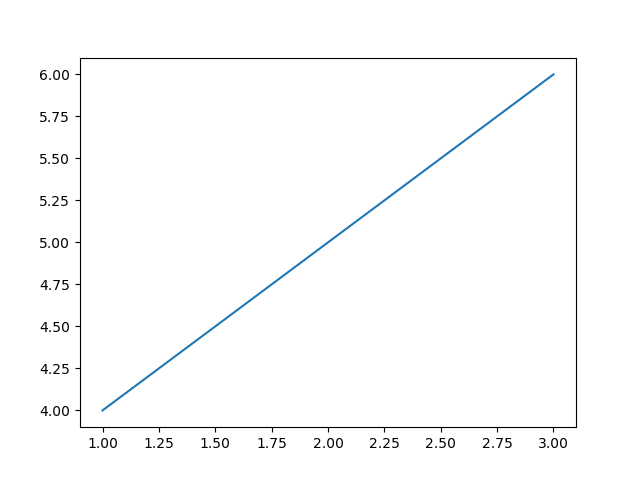
\includegraphics[width=.9\linewidth]{./quickDoc-exemple-code.png}
\caption{Résultat de l'exemple}
\end{figure}
\subsubsection{Mathématique}
\label{sec:org1fc3b94}
Pour les formules display (isolées au centre). \protect\hyperlink{gls-2}{\label{gls-2-use-12}LML} utilise également une clôture dédiée, par exemple \texttt{\$\$\$} en début et fin de bloc (analogue à \texttt{\$\$ ... \$\$} en \LaTeX{}, mais sur plusieurs lignes). Entre ces délimiteurs, on place la formule en notation \protect\hyperlink{gls-2}{\label{gls-2-use-13}LML} (très proche de la syntaxe \LaTeX{} math). Des paramètres peuvent également être fournis après les \texttt{\$\$\$} initiaux via \texttt{\{set ...\}}, notamment :
\begin{itemize}
\item solver pour spécifier un solveur si on souhaite que la formule soit calculée (ex: solver:sympy),
\item éventuellement d’autres paramètres comme le format d’affichage du résultat (exact vs numérique, nombre de décimales, etc. – ces détails pourront évoluer).
\end{itemize}

Si un solveur est indiqué, la formule sera transmise à ce solveur et son résultat (par ex. simplification ou valeur numérique) pourra être inséré soit en sus, soit à la place, selon le contexte. Par défaut, sans solver, la formule est rendue telle quelle en notation mathématique.

\begin{verbatim}
$$${<parametres>}
   <formule mathématique
   sur plusieurs
   lignes>
$$$
\end{verbatim}

Les blocs de mathématiques peuvent être associées à un résolveur d'équation tel que :
\texttt{\$\$ [[[set solver:<nom du résolveur>]]] <equation>}
Quelques exemples de résolveurs : Math.js, SymPy, Maxima, SageMath, Wolfram Alpha, etc.
\subsubsection{Commentaire}
\label{sec:org5b1929b}
\begin{description}
\item[{Commentaire}] délimiteur \texttt{;} (point-virgule) pour mettre un court commentaire non visible dans la sortie, au sein d’une phrase. Ex: \texttt{;Note interne;} sera complètement omis à l’export.
\end{description}

\textbf{quickDoc} permet des commentaires de l’auteur qui ne seront pas rendus dans la sortie finale. Ceux-ci sont noté par \texttt{;;;} en début de bloc et \texttt{;;;} en fin. Tout texte à l’intérieur est ignoré lors du rendu. Alternativement, un double point-virgule \texttt{;;} en début de ligne peut marquer un commentaire sur la ligne entière (notamment dans un bloc de code, pour commenter du code qui ne sera pas exécuté).

Des commentaires enrichis sont possibles via des paramètres type: sur le bloc de commentaire. Par exemple type:todo ou type:todo-inline pour signaler une tâche à faire. Cela pourra se traduire par un encart "TODO" visible dans le PDF/HTML, éventuellement dans la marge ou dans le flux du texte. Ceci est utile en phase de rédaction (pour indiquer des sections incomplètes, etc.).

\begin{verbatim}
;;;{<parametres>}
   <commentaires
   sur plusieurs
   lignes>
;;;
\end{verbatim}

Les blocs de commentaires sont de 4 types :
\begin{itemize}
\item sans précision, ils ne sont pas exportées
\item avec \texttt{type:todo-inline} ils impriment un bloc de type "TODO" en lieu et place ten que celui ci : \todo[inline]{bloc "TODO" en ligne}
\item avec \texttt{type:todo} ils impriment un bloc de type "TODO" dans la marge du document tel que celui ci : \todo{e.g.}
\end{itemize}
\subsubsection{Propriétés}
\label{sec:orgef64326}
Un bloc de propriété permet d’attacher des métadonnées à tout autre bloc.
\begin{itemize}
\item inline : \texttt{\{get/set prop:value\}}
\item multiline : \texttt{\{\{\{get/set prop:value\}\}\}}
\end{itemize}

Associer des propriétés à un bloc de texte :
\begin{verbatim}
Ceci est un bloc de texte avec des propriétées attachées.
{{set type:properties key1:value1 key2:value2}}
\end{verbatim}

Les propriétés peuvent être utilisés pour collecter des entrées utilisateurs et créer des formulaires en écrivant \texttt{\{get <property> <key>:<value>\}} où \texttt{<key>} correspond au type attendu et \texttt{<value>} correspond à la contrainte associée. Par exemple, voici des appels d'entrées valides :
\begin{itemize}
\item \texttt{\{get user-name string:20\}:} donnera \texttt{\_\_\_\_\_\_\_\_\_\_\_\_\_\_\_\_\_\_\_\_} et sera affecté à la propriété "user-name",
\item \texttt{\{get user-lang string:2\}} donnera \texttt{\_\_} et sera affecté à la propriété "user-lang".
\end{itemize}

Les déclarations de propriétés monoline sont de la forme \texttt{\{\{get/set prop:value\}\}}. Elles sont particulièrement adaptées à la déclaration de la mise en page du document (aligmnement du texte, mise en colonne des blocs, etc.). Ces opérations se réalisent en deux étapes : 
\begin{enumerate}
\item Définir une mise en forme tel que:
\begin{verbatim}
{{set text_style name:paraghaphe scope:raw-text al:justif size:12 long:80char color:black font:source-sans-pro columns:nil}}
\end{verbatim}
\item L'appliquer tel que:
\begin{verbatim}
{{use text-style name:paragraphe}}
\end{verbatim}
\end{enumerate}

La mise en forme sera appliquée à partir de sa déclaration (\texttt{use}) jusqu'à la déclaration d'un autre style.
\subsubsection{Tableau}
\label{sec:org98d6aae}

La syntaxe des tableaux peut s’inspirer soit de Markdown (tabulation par des \texttt{|}), soit d’AsciiDoc (lignes et colonnes séparées par \texttt{|} et formatage avancé via des cellules d’entête \texttt{!} etc.). 
Une ligne d’en-tête optionnelle, encadrée de \texttt{|} et séparant les cellules par \texttt{|}. Une ligne de séparation en-dessous composée de \texttt{|- - -|} (au moins 3 tirets entre chaque \texttt{|}) indique la fin de l’en-tête.

Puis les lignes de corps du tableau, avec la même syntaxe de cellule séparées par \texttt{|}.

\begin{verbatim}
| Colonne A | Colonne B |
|-----------+-----------|
| Valeur A1 | Valeur B1 |
| Valeur A2 | Valeur B2 |
\end{verbatim}

Les cellules peuvent contenir du texte formaté (italique, etc.) \sout{mais pas de blocs multiples (pas de titre ou liste à l’intérieur d’une cellule, sauf en utilisant éventuellement des astuces non couvertes ici).} La portée de cette spécification de tableau est \sout{limitée aux usages simples de type CSV mis en forme.} Les aspects plus complexes (fusion de cellules, tableaux imbriqués) \sout{ne sont pas gérés nativement par \protect\hyperlink{gls-2}{\label{gls-2-use-14}LML} v1, mais pourraient être ajoutés via des extensions}.
\subsubsection{Bloc sémantique}
\label{sec:org6d0c700}
utilise les \texttt{<} / \texttt{>}
\subsubsection{Multimédia}
\label{sec:org848f36c}
L’insertion d’une image se fera via une directive de lien spécialisée (voir 5.6 sur les liens). Tout lien vers un fichier image (ex: \texttt{[[img:chemin/figure.png]]}) insère l’image dans le document. Pour ajouter une légende, on pourra encapsuler cette image dans un bloc de figure, par exemple en la précédant d’un titre de figure ou en utilisant une macro dédiée. Une approche consiste à traiter une image insérée isolée avec un texte de légende suivant immédiatement comme une figure groupée. Par exemple :
\begin{verbatim}
[[img:diagrams/schéma1.svg]]  
{{{set
      id:img1
      title:"Processus illustré"
      alt-text:"Schéma illustratif du processus"
      description:"Une description factuelle de l'image"
}}}
\end{verbatim}
\subsubsection{Snippets}
\label{sec:orgdb7c6d2}
(fragments réutilisables) mécanisme permettant d’injecter du contenu ou des références (ex. inclusion de la valeur d’une propriété).

Tous les blocs de textes peuvent être associées à des tags.
Un tag s'écrit \texttt{\#<tag>} peut être insérée à n'importe quel endroit du bloc de texte en respectant les rêgles de balisage décrites au paragraphe \ref{sec:org8ed179d}.

\begin{table}[htbp]
\caption{\label{tab:org48b1840}liste des snippets}
\centering
\begin{tabular}{lll}
\hline
Type & Lemma & Behavior\\
\hline
Ref Link & \texttt{@element} & Insère un \texttt{[[lien]]} unidirectionnel\\
Tag & \texttt{\#tag} & Insère un \texttt{[[lien]]} bidirectionnel\\
\hline
\end{tabular}
\end{table}

Les tags sont utilisés pour faire de l'analyse sémantique. Ecrire un tag entraine la création ou la mise à jour d'un fichier "tag\_<nom-du-tag>.qdo" constitué comme ceci :
\begin{verbatim}
# Nom-du-tag
[[[get count:?]]] ;; nombre d'occurence dans le projet
[[[get blocs:?nom-du-tag]]] ;; tous les blocs utilisants le tag
\end{verbatim}

L'instruction \texttt{[[[get blocs:?nom-du-tag]]]} peut être complété par un système de tris. Par exemple, pour lister les blocs par ordre de date décroissante on écrira \texttt{[[[get blocs:?nom-du-tag order-by:date-desc]]]}.

Un système de trâme permettant aux utilisateurs de préconfigurer ces documents et de modifier en lot leurs configuration serait un atoût en matière d'expérience utilisateur.

Les snippets sont une fonctionnalité héritée notamment de quickDoc, permettant d’insérer dynamiquement des contenus générés ou de référencer des éléments transverses du document. Ils se présentent sous forme de balises triple-crochets avec mot-clé, par exemple \texttt{[[[get ...]]]} ou \texttt{[[[set ...]]]}.

5.5.1 \texttt{[[[set ...]]]} – définition de propriété ou configuration

La balise set est utilisée soit en tête de document pour définir des styles/config globales, soit au sein de blocs (comme vu plus haut) pour paramétrer un bloc spécifique (langage d’un code, type d’admonition, etc.). En général, \texttt{[[[set X:Y ...]]]} signifie « assigner la propriété X avec la valeur Y ». Par exemple: \texttt{[[[set color:blue]]]}. Dans le cas des blocs, cette instruction apparaît immédiatement après l’ouverture du bloc (comme illustré pour les blocs de code, de maths, etc.). Dans le cas d’une configuration globale, on peut l’utiliser soit dans le front-matter, soit sur une ligne spéciale au début du document éventuellement introduite par un commentaire. QuickDoc montrait une inclusion de fichier de config via \texttt{;;[[[set config file:...]]]}, \protect\hyperlink{gls-2}{\label{gls-2-use-15}LML} pourra avoir plus simplement dans le front-matter une section dédiée pour importer des configs.

En résumé, \texttt{[[[set ...]]]} n’est pas exactement un snippet inséré dans le texte final, mais une directive de réglage affectant le rendu ou le comportement.

5.5.2 \texttt{[[[get ...]]]} – insertion de contenu généré

La balise get permet de récupérer une valeur ou un contenu calculé. On l’utilise au sein du texte pour insérer, par exemple, la valeur d’un compteur, d’une propriété, ou le résultat d’une requête. Syntaxe générale: \texttt{[[[get <source> <clé>:<filtre>]]]}.

Exemples envisagés :

\texttt{[[[get count:?]]]} pourrait renvoyer un nombre, par ex. le nombre d’éléments correspondant à une requête (voir plus bas).

\texttt{[[[get blocs:?tag]]]} pour insérer la liste de tous les blocs taggés par \#tag (notion de tag abordée en 5.5.3).

\texttt{[[[get property nom]]]} pour insérer la valeur d’une propriété de métadonnée nommée nom définie dans le document (par ex. l’auteur ou le titre).

\texttt{[[[get date:now]]]} pour la date du jour, etc., ou d’autres fonctions.

\protect\hyperlink{gls-2}{\label{gls-2-use-16}LML} devra définir une liste de sources accessibles via get : count (compteurs), blocs (collection de blocs répondant à un critère), property/meta (métadonnées), possiblement env (variables d’environnement ou arguments de compilation), etc.

Des filtres ou paramètres peuvent affiner la requête, p. ex. \texttt{[[[get blocs:?tag order-by:date-desc]]]} pour trier les blocs taggés par date décroissante. Ce mécanisme puissant rapproche \protect\hyperlink{gls-2}{\label{gls-2-use-17}LML} d’un outil de gestion de connaissances, permettant de générer des index, des tables des matières, des listes de tâches automatiques, etc.

5.5.3 Tags et étiquetage sémantique

En \protect\hyperlink{gls-2}{\label{gls-2-use-18}LML}, on autorise l’ajout de tags à n’importe quel bloc de texte pour une classification sémantique. Un tag s’écrit \texttt{\#motcle} directement dans le texte ou en préfixe d’un bloc. Par exemple : \texttt{\#TODO} au début d’une ligne de liste de tâche, ou \texttt{\#important} dans un paragraphe. Ces tags ne sont pas affichés dans le rendu final, ou éventuellement transformés en éléments visuels discrets, mais surtout ils alimentent une indexation interne.

L’utilisation de tags combinée à \texttt{[[[get blocs:?tag]]]} permet de générer par exemple un index de tous les blocs marqués d’un tag particulier. On peut s’en servir pour : liste des TODO restants, index thématique, glossaire (tag \texttt{\#terme} sur la définition d’un terme), etc. Cette approche en fait un langage plus sémantique et orienté gestion de connaissances.

Techniquement, \protect\hyperlink{gls-2}{\label{gls-2-use-19}LML} pourrait créer en coulisse des fichiers ou des sections invisibles où sont listés les contenus par tag (comme quickDoc suggère un fichier tag\_nom.qdo généré pour chaque tag). La spécification peut rester au niveau conceptuel (il n’est pas nécessaire de normer comment c’est implémenté, juste que le résultat est comme si un tel index existait).
\subsubsection{Callouts}
\label{sec:org7ef744f}
Les callouts sont des liens bidirectionnels à l'intérieur d'un document et permettent de cibler des blocs. Ils sont utilisés pour sauter rapidement à un contenu, une note, une référence, etc.

\begin{table}[htbp]
\caption{\label{tab:org01bc674}Text callouts}
\centering
\begin{tabular}{lll}
\hline
Type & Lemma & Behavior\\
\hline
Reference & \texttt{[ref:id]} & \\
Foot Note & \texttt{[fn:id]} & \\
Quote & \texttt{[cite:id]} & \\
Figure ref & \texttt{[fig:id]} & \\
Table ref & \texttt{[tbl:id]} & \\
Code ref & \texttt{[src:id]} & \\
Header jump & \texttt{[head:id]} & \\
\hline
\end{tabular}
\end{table}
\subsubsection{Liens et références}
\label{sec:org6315060}
Les liens sont tous directionnels. 
\begin{description}
\item[{Référence interne}] plusieurs types de callouts permettent de créer des liens internes :
\begin{itemize}
\item \texttt{[ref:ID]} pour référence générique à un élément repéré par l’identifiant ID (section, figure, etc.). Cela affichera soit le numéro de l’élément (ex: “Figure 3”) soit un texte par défaut.
\item \texttt{[fig:ID]} affiche “Figure X” en liant vers l’image de nom ID.
\item \texttt{[tbl:ID]} pour “Tableau X”.
\item \texttt{[eq:ID]} (éventuellement) pour les équations numérotées “(X)”.
\item \texttt{[src:ID]} pour référencer un listing de code.
\item \texttt{[header:ID]} pour pointer vers le titre de section identifié.
\item \texttt{[cite:ID]} insère un renvois vers la bibliographie et référence l'entrée bibliographique.
\item \texttt{[fn:ID]}
\item \texttt{[rmq:ID]}
\end{itemize}

\item[{Liens externes}] La syntaxe générale des liens est \texttt{[[URL|texte]]} ou \texttt{[[URL]]} si pas de texte (affichera l’URL brute ou la ressource intégrée si reconnu). Par exemple: \texttt{[[https://example.com|site web]]} pour un lien hypertexte. Si le protocole est img: ou file: ou autre, cela peut déclencher des comportements spécifiques.
\end{description}

Tous les liens suivent l'écriture \texttt{[[<CONTEXT>:<LINK>]|[<TEXT>]]} pù seul le \texttt{<LINK>} \textbf{doit} être renseigné. Les autres éléments sont : 
\begin{itemize}
\item \texttt{<CONTEXT>} fournis des informations complémentaires pour l'affichage du lien. Cela permet de mettre en oeuvre des affichages adaptés aux images, vidéos, player de musique, flux RSS, etc.
\item \texttt{<LINK>} is the path of the resource on the World Wide Web, in a file system, or on any supported network. We can call a `Header ID` from the current document or from another one.
\item \texttt{<TEXT>} est le texte de remplacement à afficher à la place du lien.
\end{itemize}

un lien peut être attaché à des propriétés
\texttt{\{get\}} est utilisé pour renvoyer vers une section particulière du lien (un titre, un callout, etc.).
\texttt{\{set\}} est utilisé pour déclarer les éléments de descriptions et d'accessibilité.

\begin{table}[htbp]
\caption{\label{tab:org495f69f}\texttt{<LINK>} types}
\centering
\begin{tabular}{lll}
\hline
Type & Lemma & Can be used to\\
\hline
URI &  & \\
Web URL & \texttt{[[https:link]]} & Display a bookmark\\
Local File & \texttt{[[file:<path>]]} & \\
Musique & \texttt{[[:<path or url>]]} & Display a music player\\
Image & \texttt{[[img:<path or url>]]} & \\
Document & \texttt{[[doc:<path or url>]]} & Display a document viewer\\
Video & \texttt{[[vid:<path or url>]]} & Display a video player\\
Header ID & \texttt{[[id:headerId]]} & \\
RSS Flow & \texttt{[[rss:<url>]]} & Display a list of last entries\\
IRC Flow & \texttt{[[irc:<url>]]} & Display a list of last messages\\
Email & \texttt{[[mailto:<email>]]} & Display a contact form\\
\hline
\end{tabular}
\end{table}

\begin{description}
\item[{Tag}] \texttt{\#tag}
\item[{Mention}] \texttt{@someting} renvois à une personne ou à une étape d'un processus
\item[{Radiolink}] \texttt{[[[name]]]} crée un lien dynamique contextuel renvoyant chaque mentions du \texttt{name} du radiolien à la déclaratio nde celui-ci.
\end{description}
\subsection{Normailsation et i18n}
\label{sec:org2dd3833}
insertion des espaces insécables associés au divers éléments au regard des regles lexicales de chaque langues (guillemets, citations, doubles-points, etc.)
\subsection{Balisage}
\label{sec:org8ed179d}
Lists begins with a bullets that represent their meaning followed by a space. The following is supported :
\begin{itemize}
\item Ordered lists starts with \texttt{1.},
\item Unordered lists starts with \texttt{-},
\item Headers are lists too and starts with a \texttt{\#}, the number of \texttt{\#} set the level of the header.
\end{itemize}

Sublevels (nested lists) are supported for headers, ordered and unordered lists. There must be 4 spaces before the sublevel bullet.

The export \protect\hyperlink{gls-4}{\label{gls-4-use-3}backend} shall provide settings to customise desired formatting outputs of ordered lists (alpha-numeric numbering, dots, parentheses\ldots{}) 
\section{Consistency analysis}
\label{sec:org45c601e}
A consistent lightweight markup language shall have only one way to format text.

Markdown variants on the \ref{tab:org6388ea8} are limited to those listed by IANA's "Markdown Variant" \autocite{MarkdownVariants2023}. We exclude SSW and Quarto, the first one is too contextual and the second is based on Pandoc markdown.

\begin{table}[htbp]
\caption{\label{tab:org6388ea8}Text formatting consistency versus Markdown variants}
\centering
\begin{tabular}{lrrrrrrrrrrrr}
\hline
Format & Bol & Ita & OrL & UnL & Und & Hig & Str & Ver & Cod & Sup & Sub & Com\\
\hline
quickDoc & 1 & 1 & 1 & 1 & 1 & 1 & 1 & 1 & 1 & 1 & 1 & 1\\
CMD\autocite{johnmacfarlaneCommonMarkSpec2024} &  &  &  &  &  &  &  &  &  &  &  & \\
MMD\autocite{fletchert.penneyMultiMarkdownUsersGuide2023} &  &  &  &  &  &  &  &  &  &  &  & \\
GFM\autocite{GitHubFlavoredMarkdown2019} &  &  &  &  &  &  &  &  &  &  &  & \\
Pandoc\autocite{johnmacfarlanePandocUsersGuide2025} &  &  &  &  &  &  &  &  &  &  &  & \\
Fountain\autocite{SyntaxFountain} &  &  &  &  &  &  &  &  &  &  &  & \\
MD for RFCs\autocite{thomasleitnerKramdownSyntax} &  &  &  &  &  &  &  &  &  &  &  & \\
Pandoc2rfc &  &  &  &  &  &  &  &  &  &  &  & \\
MDX\autocite{PHPMarkdownExtra} &  &  &  &  &  &  &  &  &  &  &  & \\
MyST\autocite{JupyterbookMystmd2025} &  &  &  &  &  &  &  &  &  &  &  & \\
AsciiDoc &  &  &  &  &  &  &  &  &  &  &  & \\
reST &  &  &  &  &  &  &  &  &  &  &  & \\
Org-Mode &  &  &  &  &  &  &  &  &  &  &  & \\
Textile &  &  &  &  &  &  &  &  &  &  &  & \\
Djot &  &  &  &  &  &  &  &  &  &  &  & \\
Wikitext &  &  &  &  &  &  &  &  &  &  &  & \\
Creole &  &  &  &  &  &  &  &  &  &  &  & \\
txt2tags &  &  &  &  &  &  &  &  &  &  &  & \\
Setext &  &  &  &  &  &  &  &  &  &  &  & \\
\hline
\end{tabular}
\end{table}
\begin{tablenotes}
\begin{multicols}{3}\small
\begin{itemize}
  \item Bol : Bold
  \item Ita : Italique
  \item OrL : Ordered List
  \item UnL : Unordered List
  \item Und : Underline
  \item Hig : Highlight
  \item Str : Strike
  \item Ver : Verbatim
  \item Cod : Inline code
  \item Sup : Superscript
  \item Sub : Subscript
  \item Com : Comment
\end{itemize}
\end{multicols}
\end{tablenotes}
\section{Capacity analysis}
\label{sec:org5487cb2}

\section{Typesystem compatibility}
\label{sec:org1c31b4f}
\section{Conclusion}
\label{sec:orgc580352}

\clearpage
\section{Références du document}
\label{sec:org6c5a205}
\subsection{Liste des figures}
\label{sec:org6c6d046}
\renewcommand{\listfigurename}{\vspace{-2em}}
\listoffigures
\subsection{Liste des tableaux}
\label{sec:org7b2f855}
\renewcommand{\listtablename}{\vspace{-2em}}
\listoftables
\subsection{Liste des codes sources}
\label{sec:orgcbfcf26}
\renewcommand{\lstlistingname}{\vspace{-2em}}
\lstlistoflistings
\subsection{Liste des glosses}
\label{sec:org27c31b3}
\begin{multicols}{2}\small{
\textbf{\hypertarget{gls-4}{Backend}}\hspace*{1em}Couche logicielle gérant la logique métier, la gestion des données et la communication entre les applications\hspace*{.5em}\pageref{gls-4-use-1}, \pageref{gls-4-use-2}, \pageref{gls-4-use-3}

\textbf{\hypertarget{gls-23}{Interopérabilité}}\hspace*{1em}Capacité d’échanger par la présence d’un standard neutre et ouvert des données entre les différents « modèles » sans dépendre d’un acteur ou d’un outil en particulier.\hspace*{.5em}\pageref{gls-1-use-1}, \pageref{gls-1-use-2}, \pageref{gls-1-use-3}, \pageref{gls-1-use-4}

}\end{multicols}
\subsection{Liste des acronymes}
\label{sec:org10eb4af}
\begin{multicols}{2}\small{
\textbf{\hypertarget{gls-62}{AST}}\hspace*{1em}Abstract Syntaxe Tree\hspace*{.5em}\pageref{gls-3-use-1}, \pageref{gls-3-use-2}, \pageref{gls-3-use-3}, \pageref{gls-3-use-4}

\textbf{\hypertarget{gls-54}{API}}\hspace*{1em}Application Programming Interface\hspace*{.5em}\pageref{gls-5-use-1}, \pageref{gls-5-use-2}

\textbf{\hypertarget{gls-79}{BPMN}}\hspace*{1em}Business Process Model and Notation\hspace*{.5em}\pageref{gls-8-use-1}

\textbf{\hypertarget{gls-68}{BDD}}\hspace*{1em}Behavior-Driven Development\hspace*{.5em}\pageref{gls-6-use-1}

\textbf{\hypertarget{gls-208}{LML}}\hspace*{1em}Lightweight Markup Language\hspace*{.5em}\pageref{gls-2-use-1}, \pageref{gls-2-use-2}, \pageref{gls-2-use-3}, \pageref{gls-2-use-4}, \pageref{gls-2-use-5}, \pageref{gls-2-use-6}, \pageref{gls-2-use-7}, \pageref{gls-2-use-8}, \pageref{gls-2-use-9}, \pageref{gls-2-use-10}, \pageref{gls-2-use-11}, \pageref{gls-2-use-12}, \pageref{gls-2-use-13}, \pageref{gls-2-use-14}, \pageref{gls-2-use-15}, \pageref{gls-2-use-16}, \pageref{gls-2-use-17}, \pageref{gls-2-use-18}, \pageref{gls-2-use-19}

\textbf{\hypertarget{gls-348}{WBS}}\hspace*{1em}Work Breakdown Structure\hspace*{.5em}\pageref{gls-7-use-1}

}\clearpage\end{multicols}
\section{Bibliographie}
\label{sec:org9377407}
\begin{multicols}{2}\small{
\printbibliography[heading=none]
}\clearpage\end{multicols}
\end{document}
